\documentclass[twoside]{book}

% Packages required by doxygen
\usepackage{fixltx2e}
\usepackage{calc}
\usepackage{doxygen}
\usepackage[export]{adjustbox} % also loads graphicx
\usepackage{graphicx}
\usepackage[utf8]{inputenc}
\usepackage{makeidx}
\usepackage{multicol}
\usepackage{multirow}
\PassOptionsToPackage{warn}{textcomp}
\usepackage{textcomp}
\usepackage[nointegrals]{wasysym}
\usepackage[table]{xcolor}

% Font selection
\usepackage[T1]{fontenc}
\usepackage[scaled=.90]{helvet}
\usepackage{courier}
\usepackage{amssymb}
\usepackage{sectsty}
\renewcommand{\familydefault}{\sfdefault}
\allsectionsfont{%
  \fontseries{bc}\selectfont%
  \color{darkgray}%
}
\renewcommand{\DoxyLabelFont}{%
  \fontseries{bc}\selectfont%
  \color{darkgray}%
}
\newcommand{\+}{\discretionary{\mbox{\scriptsize$\hookleftarrow$}}{}{}}

% Page & text layout
\usepackage{geometry}
\geometry{%
  a4paper,%
  top=2.5cm,%
  bottom=2.5cm,%
  left=2.5cm,%
  right=2.5cm%
}
\tolerance=750
\hfuzz=15pt
\hbadness=750
\setlength{\emergencystretch}{15pt}
\setlength{\parindent}{0cm}
\setlength{\parskip}{3ex plus 2ex minus 2ex}
\makeatletter
\renewcommand{\paragraph}{%
  \@startsection{paragraph}{4}{0ex}{-1.0ex}{1.0ex}{%
    \normalfont\normalsize\bfseries\SS@parafont%
  }%
}
\renewcommand{\subparagraph}{%
  \@startsection{subparagraph}{5}{0ex}{-1.0ex}{1.0ex}{%
    \normalfont\normalsize\bfseries\SS@subparafont%
  }%
}
\makeatother

% Headers & footers
\usepackage{fancyhdr}
\pagestyle{fancyplain}
\fancyhead[LE]{\fancyplain{}{\bfseries\thepage}}
\fancyhead[CE]{\fancyplain{}{}}
\fancyhead[RE]{\fancyplain{}{\bfseries\leftmark}}
\fancyhead[LO]{\fancyplain{}{\bfseries\rightmark}}
\fancyhead[CO]{\fancyplain{}{}}
\fancyhead[RO]{\fancyplain{}{\bfseries\thepage}}
\fancyfoot[LE]{\fancyplain{}{}}
\fancyfoot[CE]{\fancyplain{}{}}
\fancyfoot[RE]{\fancyplain{}{\bfseries\scriptsize Generated by Doxygen }}
\fancyfoot[LO]{\fancyplain{}{\bfseries\scriptsize Generated by Doxygen }}
\fancyfoot[CO]{\fancyplain{}{}}
\fancyfoot[RO]{\fancyplain{}{}}
\renewcommand{\footrulewidth}{0.4pt}
\renewcommand{\chaptermark}[1]{%
  \markboth{#1}{}%
}
\renewcommand{\sectionmark}[1]{%
  \markright{\thesection\ #1}%
}

% Indices & bibliography
\usepackage{natbib}
\usepackage[titles]{tocloft}
\setcounter{tocdepth}{3}
\setcounter{secnumdepth}{5}
\makeindex

% Hyperlinks (required, but should be loaded last)
\usepackage{ifpdf}
\ifpdf
  \usepackage[pdftex,pagebackref=true]{hyperref}
\else
  \usepackage[ps2pdf,pagebackref=true]{hyperref}
\fi
\hypersetup{%
  colorlinks=true,%
  linkcolor=blue,%
  citecolor=blue,%
  unicode%
}

% Custom commands
\newcommand{\clearemptydoublepage}{%
  \newpage{\pagestyle{empty}\cleardoublepage}%
}

\usepackage{caption}
\captionsetup{labelsep=space,justification=centering,font={bf},singlelinecheck=off,skip=4pt,position=top}

%===== C O N T E N T S =====

\begin{document}

% Titlepage & ToC
\hypersetup{pageanchor=false,
             bookmarksnumbered=true,
             pdfencoding=unicode
            }
\pagenumbering{alph}
\begin{titlepage}
\vspace*{7cm}
\begin{center}%
{\Large A\+C\+ME Drone Simulation }\\
\vspace*{1cm}
{\large Generated by Doxygen 1.8.13}\\
\end{center}
\end{titlepage}
\clearemptydoublepage
\pagenumbering{roman}
\tableofcontents
\clearemptydoublepage
\pagenumbering{arabic}
\hypersetup{pageanchor=true}

%--- Begin generated contents ---
\chapter{C\+S\+CI 3081W Drone Simulation Project}
\label{index}\hypertarget{index}{}\hypertarget{index_intro_sec}{}\section{Description}\label{index_intro_sec}
This page contains supplementary documentation for our implementation of our Drone Simulation, which handles the creation, scheduling, and drone delivery of A\+C\+ME packages. 
\chapter{Hierarchical Index}
\section{Class Hierarchy}
This inheritance list is sorted roughly, but not completely, alphabetically\+:\begin{DoxyCompactList}
\item Customer\begin{DoxyCompactList}
\item \contentsline{section}{csci3081\+:\+:Customer}{\pageref{classcsci3081_1_1Customer}}{}
\end{DoxyCompactList}
\item Drone\begin{DoxyCompactList}
\item \contentsline{section}{csci3081\+:\+:Drone}{\pageref{classcsci3081_1_1Drone}}{}
\end{DoxyCompactList}
\item Drone\+Delivery\+System\begin{DoxyCompactList}
\item \contentsline{section}{csci3081\+:\+:Drone\+Simulation}{\pageref{classcsci3081_1_1DroneSimulation}}{}
\end{DoxyCompactList}
\item \contentsline{section}{csci3081\+:\+:Entity\+Creator}{\pageref{classcsci3081_1_1EntityCreator}}{}
\begin{DoxyCompactList}
\item \contentsline{section}{csci3081\+:\+:Customer\+Creator}{\pageref{classcsci3081_1_1CustomerCreator}}{}
\item \contentsline{section}{csci3081\+:\+:Drone\+Creator}{\pageref{classcsci3081_1_1DroneCreator}}{}
\item \contentsline{section}{csci3081\+:\+:Package\+Creator}{\pageref{classcsci3081_1_1PackageCreator}}{}
\end{DoxyCompactList}
\item Entity\+Observer\begin{DoxyCompactList}
\item \contentsline{section}{csci3081\+:\+:Entity\+Observer}{\pageref{classcsci3081_1_1EntityObserver}}{}
\begin{DoxyCompactList}
\item \contentsline{section}{csci3081\+:\+:Customer\+Observer}{\pageref{classcsci3081_1_1CustomerObserver}}{}
\item \contentsline{section}{csci3081\+:\+:Drone\+Observer}{\pageref{classcsci3081_1_1DroneObserver}}{}
\item \contentsline{section}{csci3081\+:\+:Package\+Observer}{\pageref{classcsci3081_1_1PackageObserver}}{}
\end{DoxyCompactList}
\end{DoxyCompactList}
\item Package\begin{DoxyCompactList}
\item \contentsline{section}{csci3081\+:\+:Package}{\pageref{classcsci3081_1_1Package}}{}
\end{DoxyCompactList}
\item \contentsline{section}{csci3081\+:\+:Scheduler}{\pageref{classcsci3081_1_1Scheduler}}{}
\end{DoxyCompactList}

\chapter{Class Index}
\section{Class List}
Here are the classes, structs, unions and interfaces with brief descriptions\+:\begin{DoxyCompactList}
\item\contentsline{section}{\hyperlink{classcsci3081_1_1Customer}{csci3081\+::\+Customer} \\*Stores data about \hyperlink{classcsci3081_1_1Customer}{Customer} entities }{\pageref{classcsci3081_1_1Customer}}{}
\item\contentsline{section}{\hyperlink{classcsci3081_1_1CustomerCreator}{csci3081\+::\+Customer\+Creator} \\*A class that creates a \hyperlink{classcsci3081_1_1Customer}{Customer} object }{\pageref{classcsci3081_1_1CustomerCreator}}{}
\item\contentsline{section}{\hyperlink{classcsci3081_1_1CustomerObserver}{csci3081\+::\+Customer\+Observer} \\*Implements \hyperlink{classcsci3081_1_1Customer}{Customer} observer }{\pageref{classcsci3081_1_1CustomerObserver}}{}
\item\contentsline{section}{\hyperlink{classcsci3081_1_1Drone}{csci3081\+::\+Drone} \\*Stores data about \hyperlink{classcsci3081_1_1Drone}{Drone} entities }{\pageref{classcsci3081_1_1Drone}}{}
\item\contentsline{section}{\hyperlink{classcsci3081_1_1DroneCreator}{csci3081\+::\+Drone\+Creator} \\*A class that creates a \hyperlink{classcsci3081_1_1Drone}{Drone} object }{\pageref{classcsci3081_1_1DroneCreator}}{}
\item\contentsline{section}{\hyperlink{classcsci3081_1_1DroneObserver}{csci3081\+::\+Drone\+Observer} \\*Implements \hyperlink{classcsci3081_1_1Drone}{Drone} observer }{\pageref{classcsci3081_1_1DroneObserver}}{}
\item\contentsline{section}{\hyperlink{classcsci3081_1_1DroneSimulation}{csci3081\+::\+Drone\+Simulation} \\*A facade class that implements the \hyperlink{classcsci3081_1_1Drone}{Drone} Delivery System }{\pageref{classcsci3081_1_1DroneSimulation}}{}
\item\contentsline{section}{\hyperlink{classcsci3081_1_1EntityCreator}{csci3081\+::\+Entity\+Creator} \\*An abstract class that creates entities }{\pageref{classcsci3081_1_1EntityCreator}}{}
\item\contentsline{section}{\hyperlink{classcsci3081_1_1EntityObserver}{csci3081\+::\+Entity\+Observer} \\*An abstract class from which specialized entity observers inherit from }{\pageref{classcsci3081_1_1EntityObserver}}{}
\item\contentsline{section}{\hyperlink{classcsci3081_1_1Package}{csci3081\+::\+Package} \\*Stores data about \hyperlink{classcsci3081_1_1Package}{Package} entities }{\pageref{classcsci3081_1_1Package}}{}
\item\contentsline{section}{\hyperlink{classcsci3081_1_1PackageCreator}{csci3081\+::\+Package\+Creator} \\*A class that creates a \hyperlink{classcsci3081_1_1Package}{Package} object }{\pageref{classcsci3081_1_1PackageCreator}}{}
\item\contentsline{section}{\hyperlink{classcsci3081_1_1PackageObserver}{csci3081\+::\+Package\+Observer} \\*Implements \hyperlink{classcsci3081_1_1Package}{Package} observer }{\pageref{classcsci3081_1_1PackageObserver}}{}
\item\contentsline{section}{\hyperlink{classcsci3081_1_1Scheduler}{csci3081\+::\+Scheduler} \\*A class that stores and handles the entities in the \hyperlink{classcsci3081_1_1DroneSimulation}{Drone\+Simulation} system }{\pageref{classcsci3081_1_1Scheduler}}{}
\end{DoxyCompactList}

\chapter{File Index}
\section{File List}
Here is a list of all documented files with brief descriptions\+:\begin{DoxyCompactList}
\item\contentsline{section}{src/\hyperlink{customer_8h}{customer.\+h} }{\pageref{customer_8h}}{}
\item\contentsline{section}{src/\hyperlink{customer__creator_8h}{customer\+\_\+creator.\+h} }{\pageref{customer__creator_8h}}{}
\item\contentsline{section}{src/\hyperlink{customer__observer_8h}{customer\+\_\+observer.\+h} }{\pageref{customer__observer_8h}}{}
\item\contentsline{section}{src/\hyperlink{drone_8h}{drone.\+h} }{\pageref{drone_8h}}{}
\item\contentsline{section}{src/\hyperlink{drone__creator_8h}{drone\+\_\+creator.\+h} }{\pageref{drone__creator_8h}}{}
\item\contentsline{section}{src/\hyperlink{drone__observer_8h}{drone\+\_\+observer.\+h} }{\pageref{drone__observer_8h}}{}
\item\contentsline{section}{src/\hyperlink{drone__simulation_8h}{drone\+\_\+simulation.\+h} }{\pageref{drone__simulation_8h}}{}
\item\contentsline{section}{src/\hyperlink{entity__creator_8h}{entity\+\_\+creator.\+h} }{\pageref{entity__creator_8h}}{}
\item\contentsline{section}{src/\hyperlink{entity__observer_8h}{entity\+\_\+observer.\+h} }{\pageref{entity__observer_8h}}{}
\item\contentsline{section}{src/{\bfseries mainpage.\+h} }{\pageref{mainpage_8h}}{}
\item\contentsline{section}{src/{\bfseries package.\+h} }{\pageref{package_8h}}{}
\item\contentsline{section}{src/\hyperlink{package__creator_8h}{package\+\_\+creator.\+h} }{\pageref{package__creator_8h}}{}
\item\contentsline{section}{src/\hyperlink{package__observer_8h}{package\+\_\+observer.\+h} }{\pageref{package__observer_8h}}{}
\item\contentsline{section}{src/\hyperlink{scheduler_8h}{scheduler.\+h} }{\pageref{scheduler_8h}}{}
\end{DoxyCompactList}

\chapter{Class Documentation}
\hypertarget{classcsci3081_1_1Customer}{}\section{csci3081\+:\+:Customer Class Reference}
\label{classcsci3081_1_1Customer}\index{csci3081\+::\+Customer@{csci3081\+::\+Customer}}


Stores data about \hyperlink{classcsci3081_1_1Customer}{Customer} entities.  




{\ttfamily \#include $<$customer.\+h$>$}



Inheritance diagram for csci3081\+:\+:Customer\+:\nopagebreak
\begin{figure}[H]
\begin{center}
\leavevmode
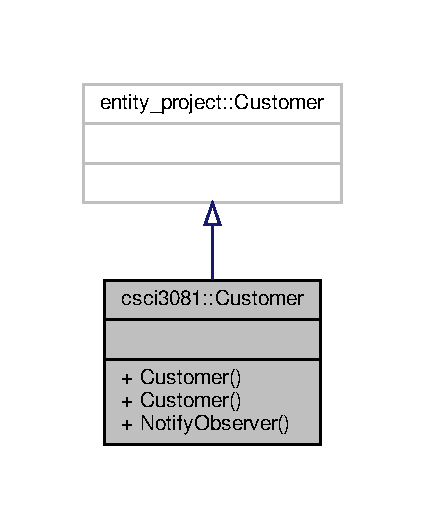
\includegraphics[width=204pt]{classcsci3081_1_1Customer__inherit__graph}
\end{center}
\end{figure}


Collaboration diagram for csci3081\+:\+:Customer\+:\nopagebreak
\begin{figure}[H]
\begin{center}
\leavevmode
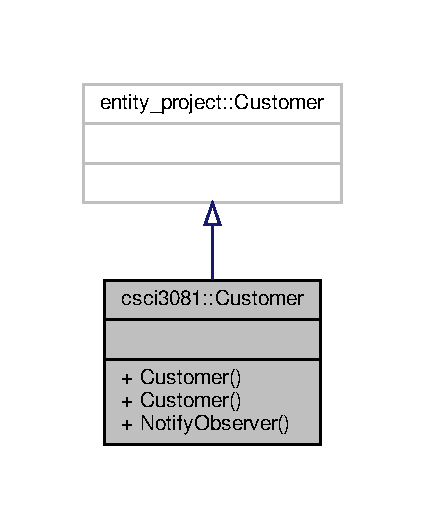
\includegraphics[width=204pt]{classcsci3081_1_1Customer__coll__graph}
\end{center}
\end{figure}
\subsection*{Public Member Functions}
\begin{DoxyCompactItemize}
\item 
\mbox{\Hypertarget{classcsci3081_1_1Customer_a070d6e1d53ddad733934c97994b104f3}\label{classcsci3081_1_1Customer_a070d6e1d53ddad733934c97994b104f3}} 
\hyperlink{classcsci3081_1_1Customer_a070d6e1d53ddad733934c97994b104f3}{Customer} ()
\begin{DoxyCompactList}\small\item\em Default constructor. \end{DoxyCompactList}\item 
\mbox{\Hypertarget{classcsci3081_1_1Customer_abbbf2b0f11d653b3cb0c2926064a830a}\label{classcsci3081_1_1Customer_abbbf2b0f11d653b3cb0c2926064a830a}} 
\hyperlink{classcsci3081_1_1Customer_abbbf2b0f11d653b3cb0c2926064a830a}{Customer} (const picojson\+::object \&val)
\begin{DoxyCompactList}\small\item\em Generates customer from picojson\+::object. \end{DoxyCompactList}\item 
\mbox{\Hypertarget{classcsci3081_1_1Customer_ae740879dfd4b71ac89bcc20d51ea3187}\label{classcsci3081_1_1Customer_ae740879dfd4b71ac89bcc20d51ea3187}} 
void \hyperlink{classcsci3081_1_1Customer_ae740879dfd4b71ac89bcc20d51ea3187}{Notify\+Observer} (std\+::string status)
\begin{DoxyCompactList}\small\item\em Notifies the observer to update status. \end{DoxyCompactList}\end{DoxyCompactItemize}


\subsection{Detailed Description}
Stores data about \hyperlink{classcsci3081_1_1Customer}{Customer} entities. 

Each \hyperlink{classcsci3081_1_1Customer}{Customer} object has its own oberver, which keeps track of whether the \hyperlink{classcsci3081_1_1Customer}{Customer} has received its package or not. 

The documentation for this class was generated from the following file\+:\begin{DoxyCompactItemize}
\item 
src/\hyperlink{customer_8h}{customer.\+h}\end{DoxyCompactItemize}

\hypertarget{classcsci3081_1_1CustomerCreator}{}\section{csci3081\+:\+:Customer\+Creator Class Reference}
\label{classcsci3081_1_1CustomerCreator}\index{csci3081\+::\+Customer\+Creator@{csci3081\+::\+Customer\+Creator}}


A class that creates a \hyperlink{classcsci3081_1_1Customer}{Customer} object.  




{\ttfamily \#include $<$customer\+\_\+creator.\+h$>$}



Inheritance diagram for csci3081\+:\+:Customer\+Creator\+:\nopagebreak
\begin{figure}[H]
\begin{center}
\leavevmode
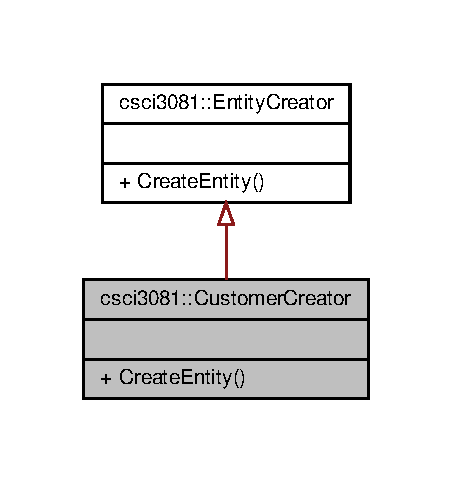
\includegraphics[width=217pt]{classcsci3081_1_1CustomerCreator__inherit__graph}
\end{center}
\end{figure}


Collaboration diagram for csci3081\+:\+:Customer\+Creator\+:\nopagebreak
\begin{figure}[H]
\begin{center}
\leavevmode
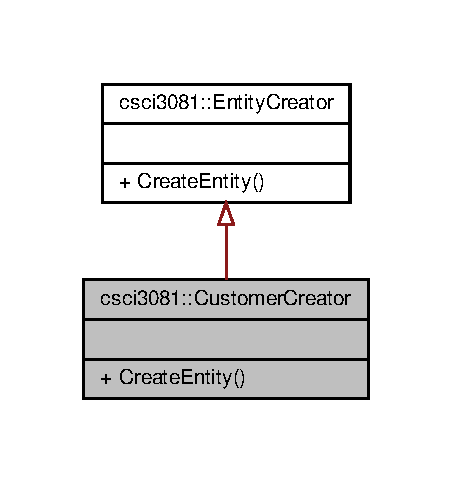
\includegraphics[width=217pt]{classcsci3081_1_1CustomerCreator__coll__graph}
\end{center}
\end{figure}
\subsection*{Public Member Functions}
\begin{DoxyCompactItemize}
\item 
\mbox{\Hypertarget{classcsci3081_1_1CustomerCreator_accb94140d70211f6ac637099656d4eda}\label{classcsci3081_1_1CustomerCreator_accb94140d70211f6ac637099656d4eda}} 
entity\+\_\+project\+::\+Entity $\ast$ \hyperlink{classcsci3081_1_1CustomerCreator_accb94140d70211f6ac637099656d4eda}{Create\+Entity} (const picojson\+::object \&val)
\begin{DoxyCompactList}\small\item\em Creates new instance of customer. \end{DoxyCompactList}\end{DoxyCompactItemize}


\subsection{Detailed Description}
A class that creates a \hyperlink{classcsci3081_1_1Customer}{Customer} object. 

The documentation for this class was generated from the following file\+:\begin{DoxyCompactItemize}
\item 
src/\hyperlink{customer__creator_8h}{customer\+\_\+creator.\+h}\end{DoxyCompactItemize}

\hypertarget{classcsci3081_1_1CustomerObserver}{}\section{csci3081\+:\+:Customer\+Observer Class Reference}
\label{classcsci3081_1_1CustomerObserver}\index{csci3081\+::\+Customer\+Observer@{csci3081\+::\+Customer\+Observer}}


implements \hyperlink{classcsci3081_1_1Customer}{Customer} observer  




{\ttfamily \#include $<$customer\+\_\+observer.\+h$>$}



Inheritance diagram for csci3081\+:\+:Customer\+Observer\+:
\nopagebreak
\begin{figure}[H]
\begin{center}
\leavevmode
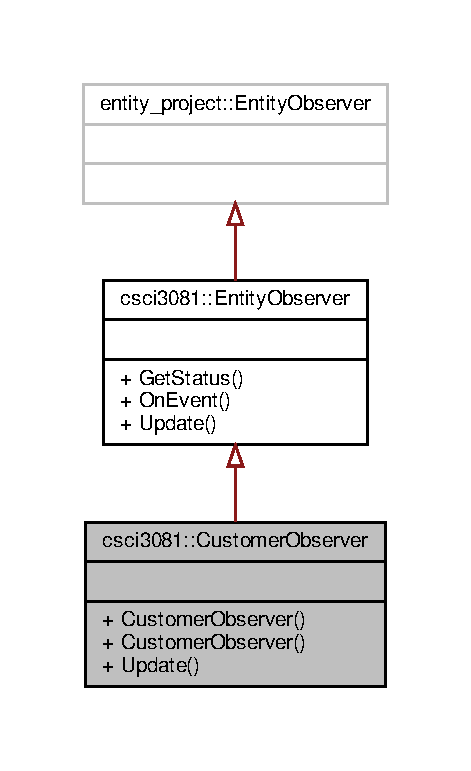
\includegraphics[width=226pt]{classcsci3081_1_1CustomerObserver__inherit__graph}
\end{center}
\end{figure}


Collaboration diagram for csci3081\+:\+:Customer\+Observer\+:
\nopagebreak
\begin{figure}[H]
\begin{center}
\leavevmode
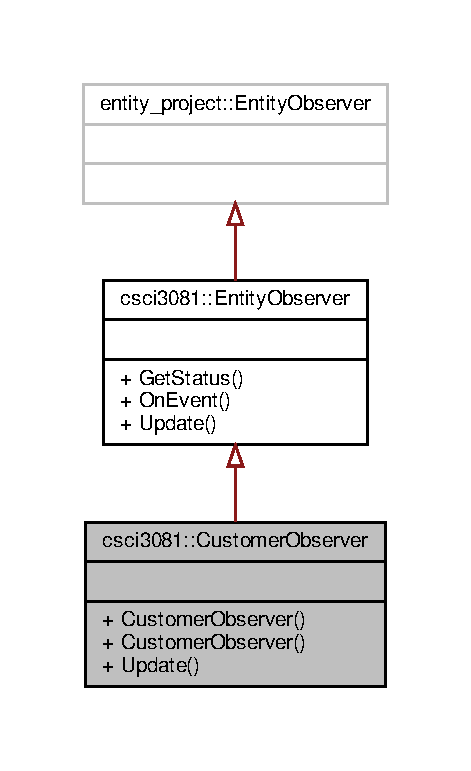
\includegraphics[width=226pt]{classcsci3081_1_1CustomerObserver__coll__graph}
\end{center}
\end{figure}
\subsection*{Public Member Functions}
\begin{DoxyCompactItemize}
\item 
\mbox{\Hypertarget{classcsci3081_1_1CustomerObserver_aef8825b1f43910c5080691d57ac2979b}\label{classcsci3081_1_1CustomerObserver_aef8825b1f43910c5080691d57ac2979b}} 
\hyperlink{classcsci3081_1_1CustomerObserver_aef8825b1f43910c5080691d57ac2979b}{Customer\+Observer} ()
\begin{DoxyCompactList}\small\item\em Default Constructor. \end{DoxyCompactList}\item 
\hyperlink{classcsci3081_1_1CustomerObserver_aa6c907db0939e504ffabfaa0a619702e}{Customer\+Observer} (entity\+\_\+project\+::\+Entity \&entity)
\begin{DoxyCompactList}\small\item\em Creates new \hyperlink{classcsci3081_1_1CustomerObserver}{Customer\+Observer} and connects it to a \hyperlink{classcsci3081_1_1Customer}{Customer} Entity. \end{DoxyCompactList}\item 
void \hyperlink{classcsci3081_1_1CustomerObserver_a2134ac33a6fd38951bbd979e6fd5a853}{Update} (std\+::string status)
\begin{DoxyCompactList}\small\item\em Alter behavior/status of drone in response to status change. \end{DoxyCompactList}\end{DoxyCompactItemize}


\subsection{Detailed Description}
implements \hyperlink{classcsci3081_1_1Customer}{Customer} observer 

\subsection{Constructor \& Destructor Documentation}
\mbox{\Hypertarget{classcsci3081_1_1CustomerObserver_aa6c907db0939e504ffabfaa0a619702e}\label{classcsci3081_1_1CustomerObserver_aa6c907db0939e504ffabfaa0a619702e}} 
\index{csci3081\+::\+Customer\+Observer@{csci3081\+::\+Customer\+Observer}!Customer\+Observer@{Customer\+Observer}}
\index{Customer\+Observer@{Customer\+Observer}!csci3081\+::\+Customer\+Observer@{csci3081\+::\+Customer\+Observer}}
\subsubsection{\texorpdfstring{Customer\+Observer()}{CustomerObserver()}}
{\footnotesize\ttfamily csci3081\+::\+Customer\+Observer\+::\+Customer\+Observer (\begin{DoxyParamCaption}\item[{entity\+\_\+project\+::\+Entity \&}]{entity }\end{DoxyParamCaption})\hspace{0.3cm}{\ttfamily [inline]}}



Creates new \hyperlink{classcsci3081_1_1CustomerObserver}{Customer\+Observer} and connects it to a \hyperlink{classcsci3081_1_1Customer}{Customer} Entity. 

Instantiates observer with status \char`\"{}\+Waiting\char`\"{} 

\subsection{Member Function Documentation}
\mbox{\Hypertarget{classcsci3081_1_1CustomerObserver_a2134ac33a6fd38951bbd979e6fd5a853}\label{classcsci3081_1_1CustomerObserver_a2134ac33a6fd38951bbd979e6fd5a853}} 
\index{csci3081\+::\+Customer\+Observer@{csci3081\+::\+Customer\+Observer}!Update@{Update}}
\index{Update@{Update}!csci3081\+::\+Customer\+Observer@{csci3081\+::\+Customer\+Observer}}
\subsubsection{\texorpdfstring{Update()}{Update()}}
{\footnotesize\ttfamily void csci3081\+::\+Customer\+Observer\+::\+Update (\begin{DoxyParamCaption}\item[{std\+::string}]{status }\end{DoxyParamCaption})\hspace{0.3cm}{\ttfamily [inline]}, {\ttfamily [virtual]}}



Alter behavior/status of drone in response to status change. 

Called by observer\textquotesingle{}s On\+Event method. 

Implements \hyperlink{classcsci3081_1_1EntityObserver_ad3188f03b6e68961ffcc415526795867}{csci3081\+::\+Entity\+Observer}.



The documentation for this class was generated from the following file\+:\begin{DoxyCompactItemize}
\item 
src/\hyperlink{customer__observer_8h}{customer\+\_\+observer.\+h}\end{DoxyCompactItemize}

\hypertarget{classcsci3081_1_1Drone}{}\section{csci3081\+:\+:Drone Class Reference}
\label{classcsci3081_1_1Drone}\index{csci3081\+::\+Drone@{csci3081\+::\+Drone}}


Stores data about \hyperlink{classcsci3081_1_1Drone}{Drone} entities.  




{\ttfamily \#include $<$drone.\+h$>$}



Inheritance diagram for csci3081\+:\+:Drone\+:\nopagebreak
\begin{figure}[H]
\begin{center}
\leavevmode
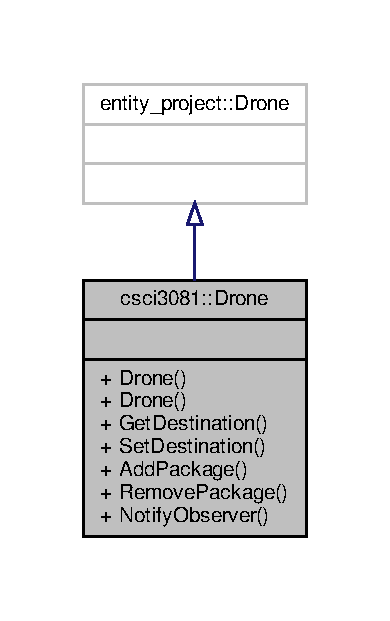
\includegraphics[width=187pt]{classcsci3081_1_1Drone__inherit__graph}
\end{center}
\end{figure}


Collaboration diagram for csci3081\+:\+:Drone\+:\nopagebreak
\begin{figure}[H]
\begin{center}
\leavevmode
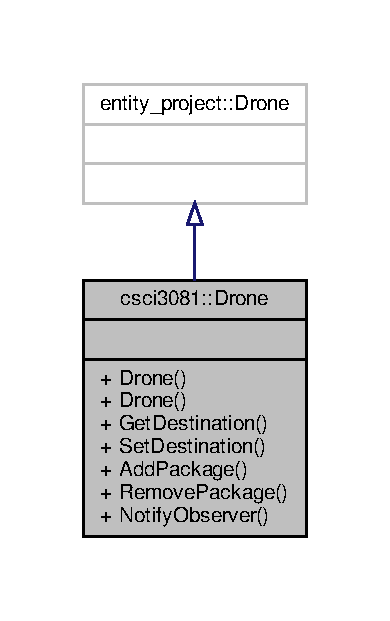
\includegraphics[width=187pt]{classcsci3081_1_1Drone__coll__graph}
\end{center}
\end{figure}
\subsection*{Public Member Functions}
\begin{DoxyCompactItemize}
\item 
\mbox{\Hypertarget{classcsci3081_1_1Drone_a7f34f6af6b978ce99ace8b15d13159c8}\label{classcsci3081_1_1Drone_a7f34f6af6b978ce99ace8b15d13159c8}} 
\hyperlink{classcsci3081_1_1Drone_a7f34f6af6b978ce99ace8b15d13159c8}{Drone} ()
\begin{DoxyCompactList}\small\item\em Default constructor. \end{DoxyCompactList}\item 
\mbox{\Hypertarget{classcsci3081_1_1Drone_ae6875af07d7f09ce59e2e2a62e5bd7d8}\label{classcsci3081_1_1Drone_ae6875af07d7f09ce59e2e2a62e5bd7d8}} 
\hyperlink{classcsci3081_1_1Drone_ae6875af07d7f09ce59e2e2a62e5bd7d8}{Drone} (const picojson\+::object \&val)
\begin{DoxyCompactList}\small\item\em Generates a drone from a picojson\+::object. \end{DoxyCompactList}\item 
\mbox{\Hypertarget{classcsci3081_1_1Drone_a888170a040c9d1138b3e57f7672efa7c}\label{classcsci3081_1_1Drone_a888170a040c9d1138b3e57f7672efa7c}} 
float $\ast$ \hyperlink{classcsci3081_1_1Drone_a888170a040c9d1138b3e57f7672efa7c}{Get\+Destination} ()
\begin{DoxyCompactList}\small\item\em Return the drone\textquotesingle{}s current destinationi. \end{DoxyCompactList}\item 
\mbox{\Hypertarget{classcsci3081_1_1Drone_acf2725b427d9e0341107096a8b7ffaf1}\label{classcsci3081_1_1Drone_acf2725b427d9e0341107096a8b7ffaf1}} 
void \hyperlink{classcsci3081_1_1Drone_acf2725b427d9e0341107096a8b7ffaf1}{Set\+Destination} (float $\ast$dest)
\begin{DoxyCompactList}\small\item\em Sets the drone\textquotesingle{}s destination. \end{DoxyCompactList}\item 
\mbox{\Hypertarget{classcsci3081_1_1Drone_a6373d2209bd49b083cffa3c2d2af9bce}\label{classcsci3081_1_1Drone_a6373d2209bd49b083cffa3c2d2af9bce}} 
int \hyperlink{classcsci3081_1_1Drone_a6373d2209bd49b083cffa3c2d2af9bce}{Add\+Package} (\hyperlink{classcsci3081_1_1Package}{Package} p)
\begin{DoxyCompactList}\small\item\em Adds package to package\+List. \end{DoxyCompactList}\item 
\mbox{\Hypertarget{classcsci3081_1_1Drone_a2b3d369000db426ad56fe5866b970544}\label{classcsci3081_1_1Drone_a2b3d369000db426ad56fe5866b970544}} 
void \hyperlink{classcsci3081_1_1Drone_a2b3d369000db426ad56fe5866b970544}{Remove\+Package} (\hyperlink{classcsci3081_1_1Package}{Package} p)
\begin{DoxyCompactList}\small\item\em Removes the specified package from package\+List, if possible. \end{DoxyCompactList}\item 
\mbox{\Hypertarget{classcsci3081_1_1Drone_a9ce811247637835a1cf8928daf95ce78}\label{classcsci3081_1_1Drone_a9ce811247637835a1cf8928daf95ce78}} 
void \hyperlink{classcsci3081_1_1Drone_a9ce811247637835a1cf8928daf95ce78}{Notify\+Observer} (std\+::string status)
\begin{DoxyCompactList}\small\item\em Notifies the observer to update the drone\textquotesingle{}s status. \end{DoxyCompactList}\end{DoxyCompactItemize}


\subsection{Detailed Description}
Stores data about \hyperlink{classcsci3081_1_1Drone}{Drone} entities. 

Drones each have a \hyperlink{classcsci3081_1_1Package}{Package} vector to store packages and a maximum capacity (weight limit). Also includes its own observer which handles the current status. 

The documentation for this class was generated from the following file\+:\begin{DoxyCompactItemize}
\item 
src/\hyperlink{drone_8h}{drone.\+h}\end{DoxyCompactItemize}

\hypertarget{classcsci3081_1_1DroneCreator}{}\section{csci3081\+:\+:Drone\+Creator Class Reference}
\label{classcsci3081_1_1DroneCreator}\index{csci3081\+::\+Drone\+Creator@{csci3081\+::\+Drone\+Creator}}


A class that creates a \hyperlink{classcsci3081_1_1Drone}{Drone} object.  




{\ttfamily \#include $<$drone\+\_\+creator.\+h$>$}



Inheritance diagram for csci3081\+:\+:Drone\+Creator\+:\nopagebreak
\begin{figure}[H]
\begin{center}
\leavevmode
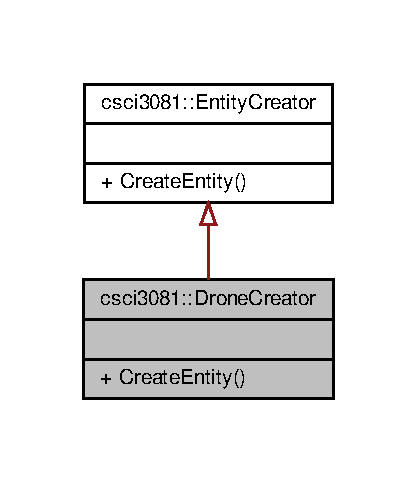
\includegraphics[width=200pt]{classcsci3081_1_1DroneCreator__inherit__graph}
\end{center}
\end{figure}


Collaboration diagram for csci3081\+:\+:Drone\+Creator\+:\nopagebreak
\begin{figure}[H]
\begin{center}
\leavevmode
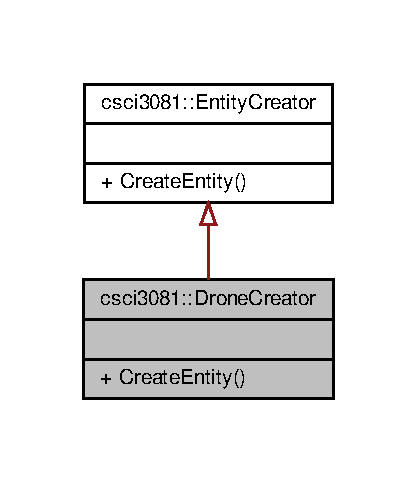
\includegraphics[width=200pt]{classcsci3081_1_1DroneCreator__coll__graph}
\end{center}
\end{figure}
\subsection*{Public Member Functions}
\begin{DoxyCompactItemize}
\item 
\mbox{\Hypertarget{classcsci3081_1_1DroneCreator_af00dafce3a19416285279d667306fc9a}\label{classcsci3081_1_1DroneCreator_af00dafce3a19416285279d667306fc9a}} 
entity\+\_\+project\+::\+Entity $\ast$ \hyperlink{classcsci3081_1_1DroneCreator_af00dafce3a19416285279d667306fc9a}{Create\+Entity} (const picojson\+::object \&val)
\begin{DoxyCompactList}\small\item\em Creates new instance of drone. \end{DoxyCompactList}\end{DoxyCompactItemize}


\subsection{Detailed Description}
A class that creates a \hyperlink{classcsci3081_1_1Drone}{Drone} object. 

The documentation for this class was generated from the following file\+:\begin{DoxyCompactItemize}
\item 
src/\hyperlink{drone__creator_8h}{drone\+\_\+creator.\+h}\end{DoxyCompactItemize}

\hypertarget{classcsci3081_1_1DroneObserver}{}\section{csci3081\+:\+:Drone\+Observer Class Reference}
\label{classcsci3081_1_1DroneObserver}\index{csci3081\+::\+Drone\+Observer@{csci3081\+::\+Drone\+Observer}}


implements \hyperlink{classcsci3081_1_1Drone}{Drone} observer  




{\ttfamily \#include $<$drone\+\_\+observer.\+h$>$}



Inheritance diagram for csci3081\+:\+:Drone\+Observer\+:\nopagebreak
\begin{figure}[H]
\begin{center}
\leavevmode
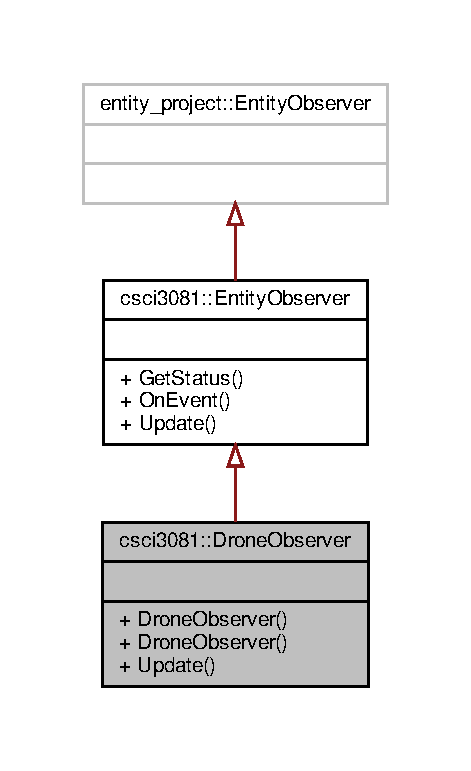
\includegraphics[width=226pt]{classcsci3081_1_1DroneObserver__inherit__graph}
\end{center}
\end{figure}


Collaboration diagram for csci3081\+:\+:Drone\+Observer\+:\nopagebreak
\begin{figure}[H]
\begin{center}
\leavevmode
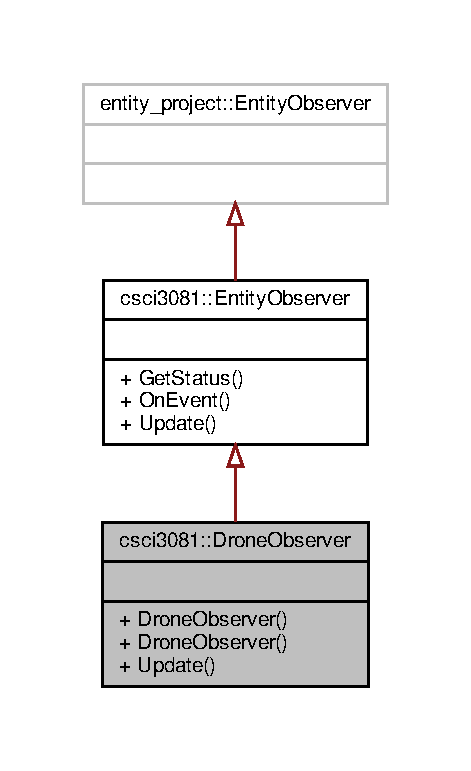
\includegraphics[width=226pt]{classcsci3081_1_1DroneObserver__coll__graph}
\end{center}
\end{figure}
\subsection*{Public Member Functions}
\begin{DoxyCompactItemize}
\item 
\mbox{\Hypertarget{classcsci3081_1_1DroneObserver_a44ea52d14f083b4b1d820bc7adf03c7a}\label{classcsci3081_1_1DroneObserver_a44ea52d14f083b4b1d820bc7adf03c7a}} 
\hyperlink{classcsci3081_1_1DroneObserver_a44ea52d14f083b4b1d820bc7adf03c7a}{Drone\+Observer} ()
\begin{DoxyCompactList}\small\item\em Default Constructor. \end{DoxyCompactList}\item 
\hyperlink{classcsci3081_1_1DroneObserver_ad065c567a9ae5d96fd69c70b45a39426}{Drone\+Observer} (entity\+\_\+project\+::\+Entity \&entity)
\begin{DoxyCompactList}\small\item\em Creates new \hyperlink{classcsci3081_1_1DroneObserver}{Drone\+Observer} and connects it to a \hyperlink{classcsci3081_1_1Drone}{Drone} Entity. \end{DoxyCompactList}\item 
void \hyperlink{classcsci3081_1_1DroneObserver_a54e1312bb116755bfa2b9a07c04632f7}{Update} (std\+::string status)
\begin{DoxyCompactList}\small\item\em Alter behavior/status of drone in response to status change. \end{DoxyCompactList}\end{DoxyCompactItemize}


\subsection{Detailed Description}
implements \hyperlink{classcsci3081_1_1Drone}{Drone} observer 

\subsection{Constructor \& Destructor Documentation}
\mbox{\Hypertarget{classcsci3081_1_1DroneObserver_ad065c567a9ae5d96fd69c70b45a39426}\label{classcsci3081_1_1DroneObserver_ad065c567a9ae5d96fd69c70b45a39426}} 
\index{csci3081\+::\+Drone\+Observer@{csci3081\+::\+Drone\+Observer}!Drone\+Observer@{Drone\+Observer}}
\index{Drone\+Observer@{Drone\+Observer}!csci3081\+::\+Drone\+Observer@{csci3081\+::\+Drone\+Observer}}
\subsubsection{\texorpdfstring{Drone\+Observer()}{DroneObserver()}}
{\footnotesize\ttfamily csci3081\+::\+Drone\+Observer\+::\+Drone\+Observer (\begin{DoxyParamCaption}\item[{entity\+\_\+project\+::\+Entity \&}]{entity }\end{DoxyParamCaption})\hspace{0.3cm}{\ttfamily [inline]}}



Creates new \hyperlink{classcsci3081_1_1DroneObserver}{Drone\+Observer} and connects it to a \hyperlink{classcsci3081_1_1Drone}{Drone} Entity. 

Instantiates observer with status \char`\"{}\+Waiting\char`\"{} 

\subsection{Member Function Documentation}
\mbox{\Hypertarget{classcsci3081_1_1DroneObserver_a54e1312bb116755bfa2b9a07c04632f7}\label{classcsci3081_1_1DroneObserver_a54e1312bb116755bfa2b9a07c04632f7}} 
\index{csci3081\+::\+Drone\+Observer@{csci3081\+::\+Drone\+Observer}!Update@{Update}}
\index{Update@{Update}!csci3081\+::\+Drone\+Observer@{csci3081\+::\+Drone\+Observer}}
\subsubsection{\texorpdfstring{Update()}{Update()}}
{\footnotesize\ttfamily void csci3081\+::\+Drone\+Observer\+::\+Update (\begin{DoxyParamCaption}\item[{std\+::string}]{status }\end{DoxyParamCaption})\hspace{0.3cm}{\ttfamily [inline]}, {\ttfamily [virtual]}}



Alter behavior/status of drone in response to status change. 

Called by observer\textquotesingle{}s On\+Event method. 

Implements \hyperlink{classcsci3081_1_1EntityObserver_ad3188f03b6e68961ffcc415526795867}{csci3081\+::\+Entity\+Observer}.



The documentation for this class was generated from the following file\+:\begin{DoxyCompactItemize}
\item 
src/\hyperlink{drone__observer_8h}{drone\+\_\+observer.\+h}\end{DoxyCompactItemize}

\hypertarget{classcsci3081_1_1DroneSimulation}{}\section{csci3081\+:\+:Drone\+Simulation Class Reference}
\label{classcsci3081_1_1DroneSimulation}\index{csci3081\+::\+Drone\+Simulation@{csci3081\+::\+Drone\+Simulation}}


A facade class that implements the \hyperlink{classcsci3081_1_1Drone}{Drone} Delivery System.  




{\ttfamily \#include $<$drone\+\_\+simulation.\+h$>$}



Inheritance diagram for csci3081\+:\+:Drone\+Simulation\+:\nopagebreak
\begin{figure}[H]
\begin{center}
\leavevmode
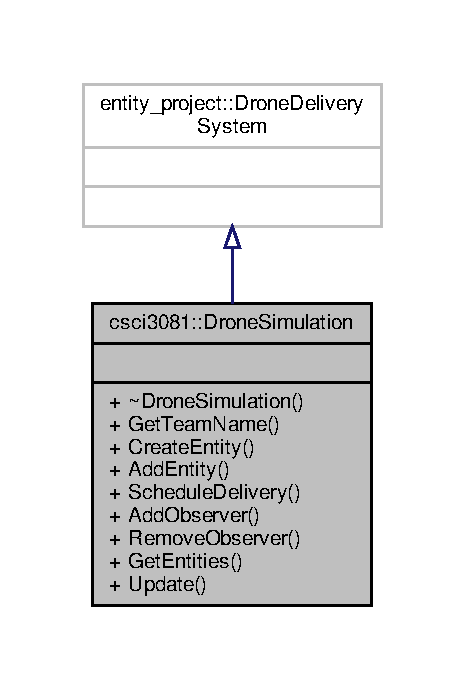
\includegraphics[width=223pt]{classcsci3081_1_1DroneSimulation__inherit__graph}
\end{center}
\end{figure}


Collaboration diagram for csci3081\+:\+:Drone\+Simulation\+:\nopagebreak
\begin{figure}[H]
\begin{center}
\leavevmode
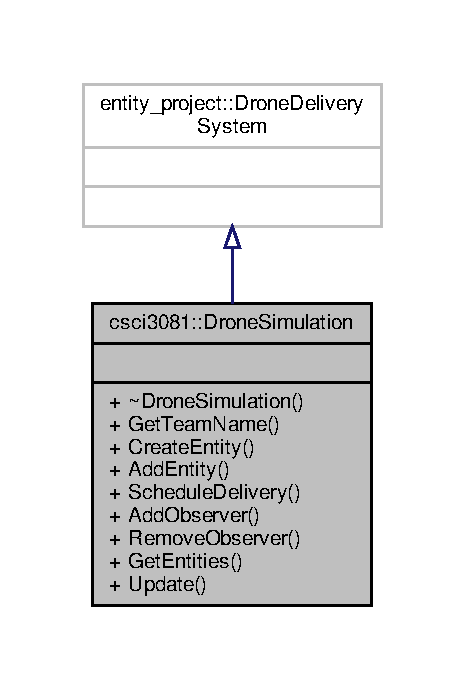
\includegraphics[width=223pt]{classcsci3081_1_1DroneSimulation__coll__graph}
\end{center}
\end{figure}
\subsection*{Public Member Functions}
\begin{DoxyCompactItemize}
\item 
\mbox{\Hypertarget{classcsci3081_1_1DroneSimulation_ab920d19a82bc4bb42722bffa3a6d0e6a}\label{classcsci3081_1_1DroneSimulation_ab920d19a82bc4bb42722bffa3a6d0e6a}} 
const std\+::string \& \hyperlink{classcsci3081_1_1DroneSimulation_ab920d19a82bc4bb42722bffa3a6d0e6a}{Get\+Team\+Name} () const
\begin{DoxyCompactList}\small\item\em Return name of the project team. \end{DoxyCompactList}\item 
entity\+\_\+project\+::\+Entity $\ast$ \hyperlink{classcsci3081_1_1DroneSimulation_af969b43abab98c458a50cad9f99a0440}{Create\+Entity} (const picojson\+::object \&val)
\begin{DoxyCompactList}\small\item\em Create an entity of type specified by J\+S\+ON object. \end{DoxyCompactList}\item 
\mbox{\Hypertarget{classcsci3081_1_1DroneSimulation_a197a3495b53ffd8041a94000eb799ef7}\label{classcsci3081_1_1DroneSimulation_a197a3495b53ffd8041a94000eb799ef7}} 
void \hyperlink{classcsci3081_1_1DroneSimulation_a197a3495b53ffd8041a94000eb799ef7}{Add\+Entity} (entity\+\_\+project\+::\+Entity $\ast$entity)
\begin{DoxyCompactList}\small\item\em Add an already created entity into the system. \end{DoxyCompactList}\item 
\mbox{\Hypertarget{classcsci3081_1_1DroneSimulation_a40816c8cef31df37015b54cc3f5015c3}\label{classcsci3081_1_1DroneSimulation_a40816c8cef31df37015b54cc3f5015c3}} 
void \hyperlink{classcsci3081_1_1DroneSimulation_a40816c8cef31df37015b54cc3f5015c3}{Schedule\+Delivery} (entity\+\_\+project\+::\+Package $\ast$package, entity\+\_\+project\+::\+Customer $\ast$dest, const picojson\+::object \&details)
\begin{DoxyCompactList}\small\item\em Schedule a drone delivery for a package to a customer. Handled by \hyperlink{classcsci3081_1_1Scheduler}{Scheduler} class. \end{DoxyCompactList}\item 
\mbox{\Hypertarget{classcsci3081_1_1DroneSimulation_a4e82dd6f5f354564e06b59d82c2056f8}\label{classcsci3081_1_1DroneSimulation_a4e82dd6f5f354564e06b59d82c2056f8}} 
void \hyperlink{classcsci3081_1_1DroneSimulation_a4e82dd6f5f354564e06b59d82c2056f8}{Add\+Observer} (entity\+\_\+project\+::\+Entity $\ast$entity, entity\+\_\+project\+::\+Entity\+Observer $\ast$observer)
\begin{DoxyCompactList}\small\item\em Add an observer to a specific entity. \end{DoxyCompactList}\item 
\mbox{\Hypertarget{classcsci3081_1_1DroneSimulation_ab796fda32c7fcd8d74e9971baf5cd608}\label{classcsci3081_1_1DroneSimulation_ab796fda32c7fcd8d74e9971baf5cd608}} 
void \hyperlink{classcsci3081_1_1DroneSimulation_ab796fda32c7fcd8d74e9971baf5cd608}{Remove\+Observer} (entity\+\_\+project\+::\+Entity $\ast$entity, entity\+\_\+project\+::\+Entity\+Observer $\ast$observer)
\begin{DoxyCompactList}\small\item\em Remove an observer from a specific entity. \end{DoxyCompactList}\item 
\mbox{\Hypertarget{classcsci3081_1_1DroneSimulation_aa9de1fa9d2090000445a093bea37ded3}\label{classcsci3081_1_1DroneSimulation_aa9de1fa9d2090000445a093bea37ded3}} 
const std\+::vector$<$ entity\+\_\+project\+::\+Entity $\ast$ $>$ \& \hyperlink{classcsci3081_1_1DroneSimulation_aa9de1fa9d2090000445a093bea37ded3}{Get\+Entities} () const
\begin{DoxyCompactList}\small\item\em Return all of the entities added into the system. \end{DoxyCompactList}\item 
\mbox{\Hypertarget{classcsci3081_1_1DroneSimulation_a17933be5048c3c2cfbcee77366bf87b9}\label{classcsci3081_1_1DroneSimulation_a17933be5048c3c2cfbcee77366bf87b9}} 
void \hyperlink{classcsci3081_1_1DroneSimulation_a17933be5048c3c2cfbcee77366bf87b9}{Update} (float dt)
\begin{DoxyCompactList}\small\item\em Updates the drone system time by dt. \end{DoxyCompactList}\end{DoxyCompactItemize}


\subsection{Detailed Description}
A facade class that implements the \hyperlink{classcsci3081_1_1Drone}{Drone} Delivery System. 

Inherits from the entity\+\_\+project\+::\+Drone\+Delivery\+System. Currently does not add any new methods or attributes, but merely implements the functions described in the entity\+\_\+project\+::\+Drone\+Delivery\+System superclass. 

\subsection{Member Function Documentation}
\mbox{\Hypertarget{classcsci3081_1_1DroneSimulation_af969b43abab98c458a50cad9f99a0440}\label{classcsci3081_1_1DroneSimulation_af969b43abab98c458a50cad9f99a0440}} 
\index{csci3081\+::\+Drone\+Simulation@{csci3081\+::\+Drone\+Simulation}!Create\+Entity@{Create\+Entity}}
\index{Create\+Entity@{Create\+Entity}!csci3081\+::\+Drone\+Simulation@{csci3081\+::\+Drone\+Simulation}}
\subsubsection{\texorpdfstring{Create\+Entity()}{CreateEntity()}}
{\footnotesize\ttfamily entity\+\_\+project\+::\+Entity$\ast$ csci3081\+::\+Drone\+Simulation\+::\+Create\+Entity (\begin{DoxyParamCaption}\item[{const picojson\+::object \&}]{val }\end{DoxyParamCaption})\hspace{0.3cm}{\ttfamily [inline]}}



Create an entity of type specified by J\+S\+ON object. 

\begin{DoxyReturn}{Returns}
the created entity object 
\end{DoxyReturn}


The documentation for this class was generated from the following file\+:\begin{DoxyCompactItemize}
\item 
src/\hyperlink{drone__simulation_8h}{drone\+\_\+simulation.\+h}\end{DoxyCompactItemize}

\hypertarget{classcsci3081_1_1EntityCreator}{}\section{csci3081\+:\+:Entity\+Creator Class Reference}
\label{classcsci3081_1_1EntityCreator}\index{csci3081\+::\+Entity\+Creator@{csci3081\+::\+Entity\+Creator}}


An abstract class that creates entities.  




{\ttfamily \#include $<$entity\+\_\+creator.\+h$>$}



Inheritance diagram for csci3081\+:\+:Entity\+Creator\+:\nopagebreak
\begin{figure}[H]
\begin{center}
\leavevmode
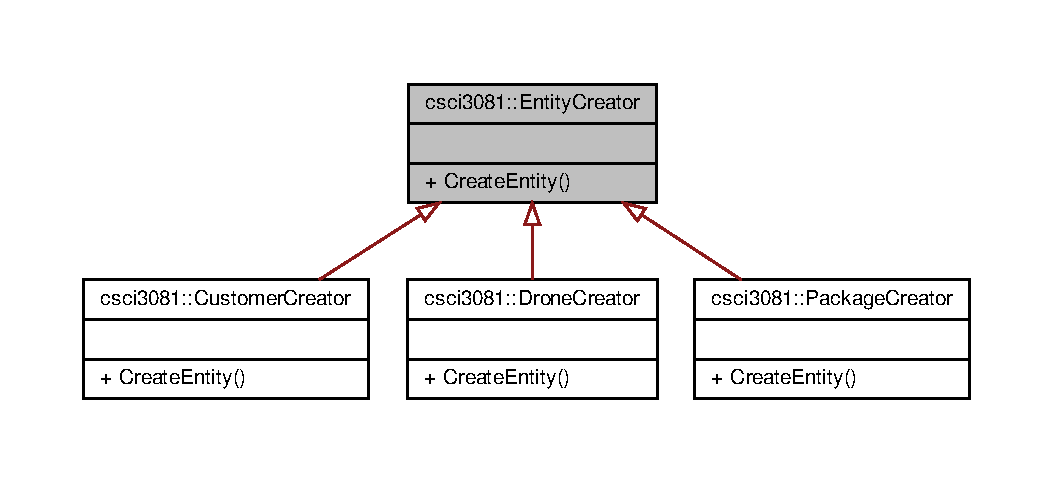
\includegraphics[width=350pt]{classcsci3081_1_1EntityCreator__inherit__graph}
\end{center}
\end{figure}


Collaboration diagram for csci3081\+:\+:Entity\+Creator\+:\nopagebreak
\begin{figure}[H]
\begin{center}
\leavevmode
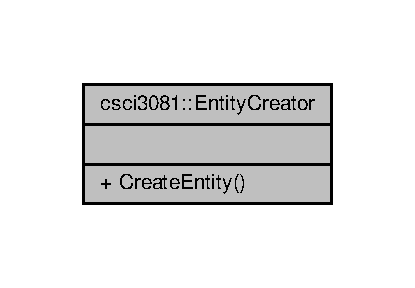
\includegraphics[width=199pt]{classcsci3081_1_1EntityCreator__coll__graph}
\end{center}
\end{figure}
\subsection*{Public Member Functions}
\begin{DoxyCompactItemize}
\item 
\mbox{\Hypertarget{classcsci3081_1_1EntityCreator_a68aab88afd1c9492be723fb852818e7f}\label{classcsci3081_1_1EntityCreator_a68aab88afd1c9492be723fb852818e7f}} 
virtual entity\+\_\+project\+::\+Entity $\ast$ \hyperlink{classcsci3081_1_1EntityCreator_a68aab88afd1c9492be723fb852818e7f}{Create\+Entity} (const picojson\+::object \&val)=0
\begin{DoxyCompactList}\small\item\em Creates and returns entity object of type specified in J\+S\+ON. \end{DoxyCompactList}\end{DoxyCompactItemize}


\subsection{Detailed Description}
An abstract class that creates entities. 

The documentation for this class was generated from the following file\+:\begin{DoxyCompactItemize}
\item 
src/\hyperlink{entity__creator_8h}{entity\+\_\+creator.\+h}\end{DoxyCompactItemize}

\hypertarget{classcsci3081_1_1EntityObserver}{}\section{csci3081\+:\+:Entity\+Observer Class Reference}
\label{classcsci3081_1_1EntityObserver}\index{csci3081\+::\+Entity\+Observer@{csci3081\+::\+Entity\+Observer}}


An abstract class from which specialized entity observers inherit from.  




{\ttfamily \#include $<$entity\+\_\+observer.\+h$>$}



Inheritance diagram for csci3081\+:\+:Entity\+Observer\+:
\nopagebreak
\begin{figure}[H]
\begin{center}
\leavevmode
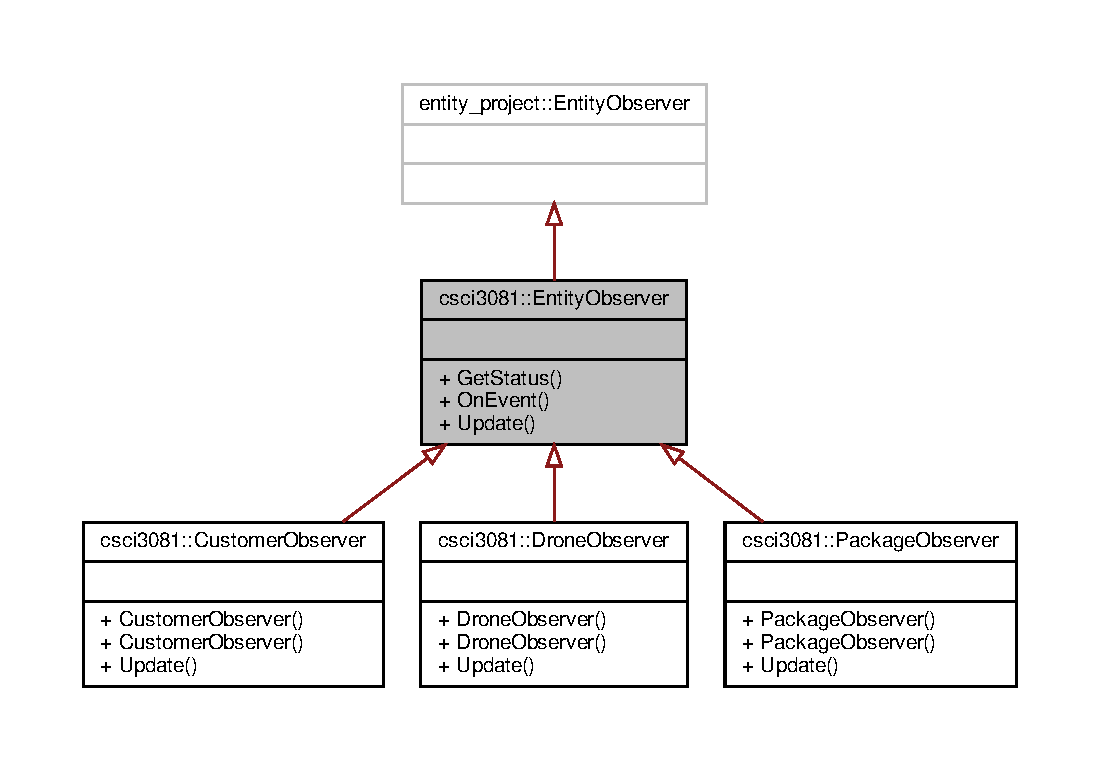
\includegraphics[width=350pt]{classcsci3081_1_1EntityObserver__inherit__graph}
\end{center}
\end{figure}


Collaboration diagram for csci3081\+:\+:Entity\+Observer\+:\nopagebreak
\begin{figure}[H]
\begin{center}
\leavevmode
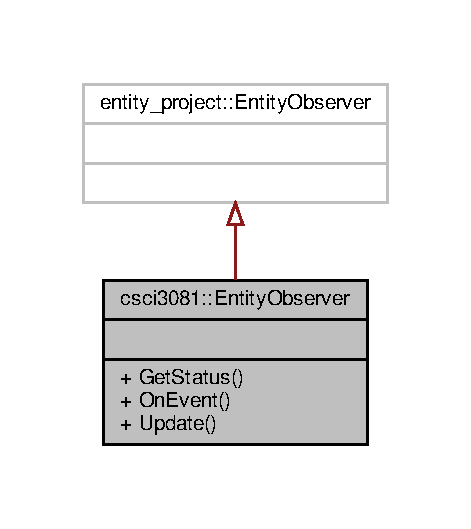
\includegraphics[width=226pt]{classcsci3081_1_1EntityObserver__coll__graph}
\end{center}
\end{figure}
\subsection*{Public Member Functions}
\begin{DoxyCompactItemize}
\item 
\mbox{\Hypertarget{classcsci3081_1_1EntityObserver_a7585beb5fe2288721f2e6d6a801cde69}\label{classcsci3081_1_1EntityObserver_a7585beb5fe2288721f2e6d6a801cde69}} 
std\+::string \hyperlink{classcsci3081_1_1EntityObserver_a7585beb5fe2288721f2e6d6a801cde69}{Get\+Status} ()
\begin{DoxyCompactList}\small\item\em Return current status of entity. \end{DoxyCompactList}\item 
int \hyperlink{classcsci3081_1_1EntityObserver_a5f972497c62a6eb6581e32fa21afbc2f}{On\+Event} (const picojson\+::value \&event, const Entity \&entity)
\begin{DoxyCompactList}\small\item\em Updates the entity\textquotesingle{}s status. \end{DoxyCompactList}\item 
virtual void \hyperlink{classcsci3081_1_1EntityObserver_ad3188f03b6e68961ffcc415526795867}{Update} (std\+::string status)=0
\begin{DoxyCompactList}\small\item\em make observer/entity react to update \end{DoxyCompactList}\end{DoxyCompactItemize}


\subsection{Detailed Description}
An abstract class from which specialized entity observers inherit from. 

\subsection{Member Function Documentation}
\mbox{\Hypertarget{classcsci3081_1_1EntityObserver_a5f972497c62a6eb6581e32fa21afbc2f}\label{classcsci3081_1_1EntityObserver_a5f972497c62a6eb6581e32fa21afbc2f}} 
\index{csci3081\+::\+Entity\+Observer@{csci3081\+::\+Entity\+Observer}!On\+Event@{On\+Event}}
\index{On\+Event@{On\+Event}!csci3081\+::\+Entity\+Observer@{csci3081\+::\+Entity\+Observer}}
\subsubsection{\texorpdfstring{On\+Event()}{OnEvent()}}
{\footnotesize\ttfamily int csci3081\+::\+Entity\+Observer\+::\+On\+Event (\begin{DoxyParamCaption}\item[{const picojson\+::value \&}]{event,  }\item[{const Entity \&}]{entity }\end{DoxyParamCaption})\hspace{0.3cm}{\ttfamily [inline]}}



Updates the entity\textquotesingle{}s status. 

Converts picojson object into string, to be stored in status\+\_\+. Then calls Update method to do something to respond to the new status.

\begin{DoxyReturn}{Returns}
1 if status successfully changed, 0 if not. 
\end{DoxyReturn}
\mbox{\Hypertarget{classcsci3081_1_1EntityObserver_ad3188f03b6e68961ffcc415526795867}\label{classcsci3081_1_1EntityObserver_ad3188f03b6e68961ffcc415526795867}} 
\index{csci3081\+::\+Entity\+Observer@{csci3081\+::\+Entity\+Observer}!Update@{Update}}
\index{Update@{Update}!csci3081\+::\+Entity\+Observer@{csci3081\+::\+Entity\+Observer}}
\subsubsection{\texorpdfstring{Update()}{Update()}}
{\footnotesize\ttfamily virtual void csci3081\+::\+Entity\+Observer\+::\+Update (\begin{DoxyParamCaption}\item[{std\+::string}]{status }\end{DoxyParamCaption})\hspace{0.3cm}{\ttfamily [pure virtual]}}



make observer/entity react to update 

Specific implementation depends on entity type and status, to be implemented in specialized observer classes. 

Implemented in \hyperlink{classcsci3081_1_1DroneObserver_a54e1312bb116755bfa2b9a07c04632f7}{csci3081\+::\+Drone\+Observer}, \hyperlink{classcsci3081_1_1PackageObserver_a8ebc5b23b82ee2a2d0ec13872f24fb6c}{csci3081\+::\+Package\+Observer}, and \hyperlink{classcsci3081_1_1CustomerObserver_a2134ac33a6fd38951bbd979e6fd5a853}{csci3081\+::\+Customer\+Observer}.



The documentation for this class was generated from the following file\+:\begin{DoxyCompactItemize}
\item 
src/\hyperlink{entity__observer_8h}{entity\+\_\+observer.\+h}\end{DoxyCompactItemize}

\hypertarget{classcsci3081_1_1Package}{}\section{csci3081\+:\+:Package Class Reference}
\label{classcsci3081_1_1Package}\index{csci3081\+::\+Package@{csci3081\+::\+Package}}


Stores data about \hyperlink{classcsci3081_1_1Package}{Package} entities.  




{\ttfamily \#include $<$package.\+h$>$}



Inheritance diagram for csci3081\+:\+:Package\+:\nopagebreak
\begin{figure}[H]
\begin{center}
\leavevmode
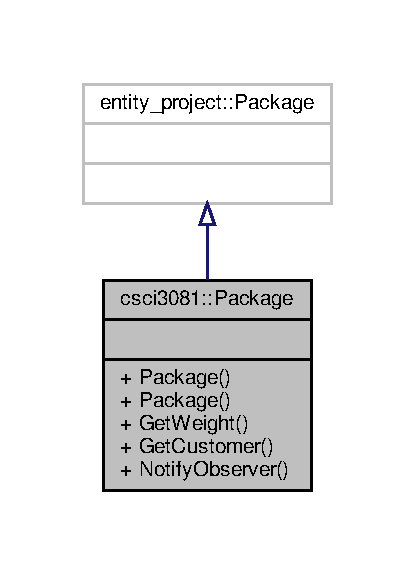
\includegraphics[width=199pt]{classcsci3081_1_1Package__inherit__graph}
\end{center}
\end{figure}


Collaboration diagram for csci3081\+:\+:Package\+:\nopagebreak
\begin{figure}[H]
\begin{center}
\leavevmode
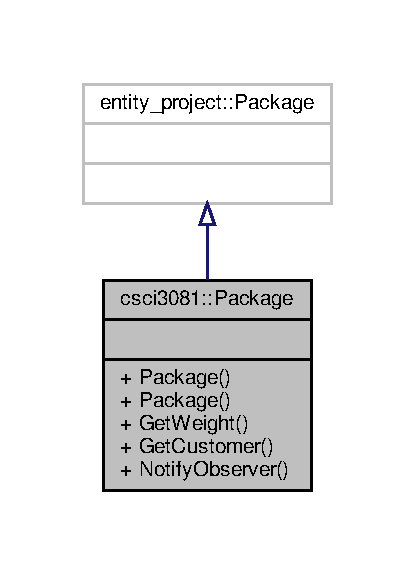
\includegraphics[width=199pt]{classcsci3081_1_1Package__coll__graph}
\end{center}
\end{figure}
\subsection*{Public Member Functions}
\begin{DoxyCompactItemize}
\item 
\mbox{\Hypertarget{classcsci3081_1_1Package_a3be008ddf9372479ce719c2e823e368e}\label{classcsci3081_1_1Package_a3be008ddf9372479ce719c2e823e368e}} 
\hyperlink{classcsci3081_1_1Package_a3be008ddf9372479ce719c2e823e368e}{Package} ()
\begin{DoxyCompactList}\small\item\em Default constructor. \end{DoxyCompactList}\item 
\mbox{\Hypertarget{classcsci3081_1_1Package_ad4665f319d2ebf5cdf9de133f0f476b3}\label{classcsci3081_1_1Package_ad4665f319d2ebf5cdf9de133f0f476b3}} 
\hyperlink{classcsci3081_1_1Package_ad4665f319d2ebf5cdf9de133f0f476b3}{Package} (const picojson\+::object \&val)
\begin{DoxyCompactList}\small\item\em Generates a package from a picojson\+::object. \end{DoxyCompactList}\item 
\mbox{\Hypertarget{classcsci3081_1_1Package_a34cb292d5b89e61724b1f8f885cc71cc}\label{classcsci3081_1_1Package_a34cb292d5b89e61724b1f8f885cc71cc}} 
double \hyperlink{classcsci3081_1_1Package_a34cb292d5b89e61724b1f8f885cc71cc}{Get\+Weight} ()
\begin{DoxyCompactList}\small\item\em Returns weight of package. \end{DoxyCompactList}\item 
\mbox{\Hypertarget{classcsci3081_1_1Package_a4f9452af878f2f119ab98b6a460afce2}\label{classcsci3081_1_1Package_a4f9452af878f2f119ab98b6a460afce2}} 
\hyperlink{classcsci3081_1_1Customer}{Customer} $\ast$ \hyperlink{classcsci3081_1_1Package_a4f9452af878f2f119ab98b6a460afce2}{Get\+Customer} ()
\begin{DoxyCompactList}\small\item\em Returns a pointer to the package\textquotesingle{}s customer. \end{DoxyCompactList}\item 
\mbox{\Hypertarget{classcsci3081_1_1Package_a0d19deea6561850c95c6c4837b1a6b43}\label{classcsci3081_1_1Package_a0d19deea6561850c95c6c4837b1a6b43}} 
void \hyperlink{classcsci3081_1_1Package_a0d19deea6561850c95c6c4837b1a6b43}{Notify\+Observer} (std\+::string status)
\begin{DoxyCompactList}\small\item\em Notifies the observer to update the package\textquotesingle{}s status. \end{DoxyCompactList}\end{DoxyCompactItemize}


\subsection{Detailed Description}
Stores data about \hyperlink{classcsci3081_1_1Package}{Package} entities. 

Packages each have a customer, a weight, and includes a \hyperlink{classcsci3081_1_1PackageObserver}{Package\+Observer}. 

The documentation for this class was generated from the following file\+:\begin{DoxyCompactItemize}
\item 
src/package.\+h\end{DoxyCompactItemize}

\hypertarget{classcsci3081_1_1PackageCreator}{}\section{csci3081\+:\+:Package\+Creator Class Reference}
\label{classcsci3081_1_1PackageCreator}\index{csci3081\+::\+Package\+Creator@{csci3081\+::\+Package\+Creator}}


A class that creates a \hyperlink{classcsci3081_1_1Package}{Package} object.  




{\ttfamily \#include $<$package\+\_\+creator.\+h$>$}



Inheritance diagram for csci3081\+:\+:Package\+Creator\+:\nopagebreak
\begin{figure}[H]
\begin{center}
\leavevmode
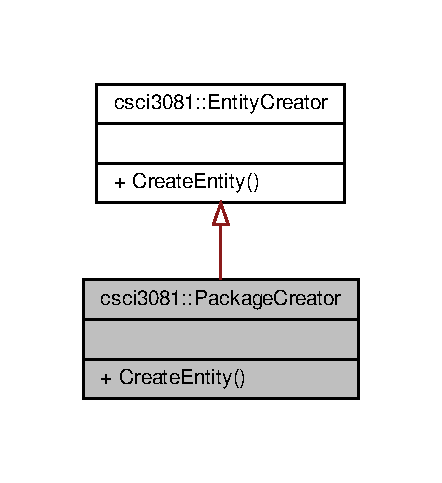
\includegraphics[width=212pt]{classcsci3081_1_1PackageCreator__inherit__graph}
\end{center}
\end{figure}


Collaboration diagram for csci3081\+:\+:Package\+Creator\+:\nopagebreak
\begin{figure}[H]
\begin{center}
\leavevmode
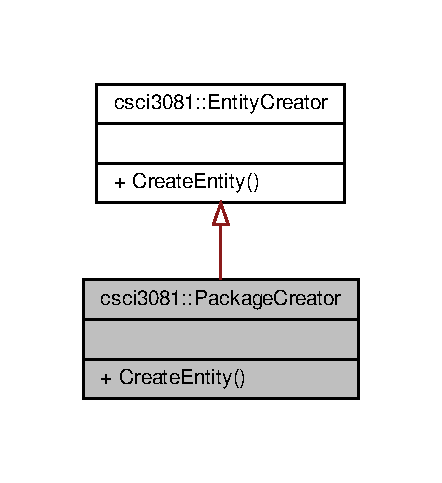
\includegraphics[width=212pt]{classcsci3081_1_1PackageCreator__coll__graph}
\end{center}
\end{figure}
\subsection*{Public Member Functions}
\begin{DoxyCompactItemize}
\item 
\mbox{\Hypertarget{classcsci3081_1_1PackageCreator_ab10a0e955c3b726cab5630e5a2b3b5bb}\label{classcsci3081_1_1PackageCreator_ab10a0e955c3b726cab5630e5a2b3b5bb}} 
entity\+\_\+project\+::\+Entity $\ast$ \hyperlink{classcsci3081_1_1PackageCreator_ab10a0e955c3b726cab5630e5a2b3b5bb}{Create\+Entity} (const picojson\+::object \&val)
\begin{DoxyCompactList}\small\item\em Creates new instance of package. \end{DoxyCompactList}\end{DoxyCompactItemize}


\subsection{Detailed Description}
A class that creates a \hyperlink{classcsci3081_1_1Package}{Package} object. 

The documentation for this class was generated from the following file\+:\begin{DoxyCompactItemize}
\item 
src/\hyperlink{package__creator_8h}{package\+\_\+creator.\+h}\end{DoxyCompactItemize}

\hypertarget{classcsci3081_1_1PackageObserver}{}\section{csci3081\+:\+:Package\+Observer Class Reference}
\label{classcsci3081_1_1PackageObserver}\index{csci3081\+::\+Package\+Observer@{csci3081\+::\+Package\+Observer}}


implements \hyperlink{classcsci3081_1_1Package}{Package} observer  




{\ttfamily \#include $<$package\+\_\+observer.\+h$>$}



Inheritance diagram for csci3081\+:\+:Package\+Observer\+:\nopagebreak
\begin{figure}[H]
\begin{center}
\leavevmode
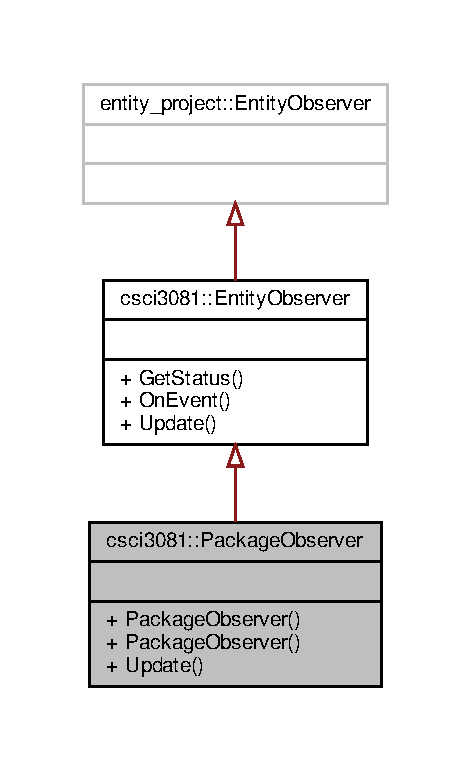
\includegraphics[width=226pt]{classcsci3081_1_1PackageObserver__inherit__graph}
\end{center}
\end{figure}


Collaboration diagram for csci3081\+:\+:Package\+Observer\+:\nopagebreak
\begin{figure}[H]
\begin{center}
\leavevmode
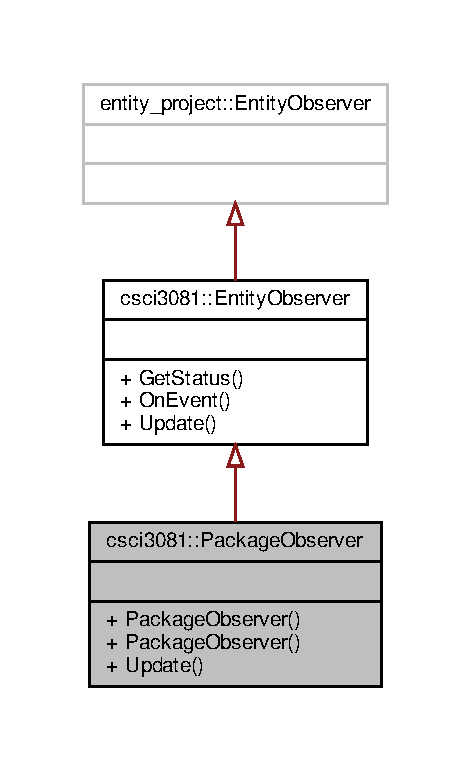
\includegraphics[width=226pt]{classcsci3081_1_1PackageObserver__coll__graph}
\end{center}
\end{figure}
\subsection*{Public Member Functions}
\begin{DoxyCompactItemize}
\item 
\mbox{\Hypertarget{classcsci3081_1_1PackageObserver_af2b41fe1a6a326362f93a12bb798d0d5}\label{classcsci3081_1_1PackageObserver_af2b41fe1a6a326362f93a12bb798d0d5}} 
\hyperlink{classcsci3081_1_1PackageObserver_af2b41fe1a6a326362f93a12bb798d0d5}{Package\+Observer} ()
\begin{DoxyCompactList}\small\item\em Default Constructor. \end{DoxyCompactList}\item 
\hyperlink{classcsci3081_1_1PackageObserver_a053e974efd7433e5b92012e68b1aee42}{Package\+Observer} (entity\+\_\+project\+::\+Entity \&entity)
\begin{DoxyCompactList}\small\item\em Creates new \hyperlink{classcsci3081_1_1PackageObserver}{Package\+Observer} and connects it to a \hyperlink{classcsci3081_1_1Package}{Package} Entity. \end{DoxyCompactList}\item 
void \hyperlink{classcsci3081_1_1PackageObserver_a8ebc5b23b82ee2a2d0ec13872f24fb6c}{Update} (std\+::string status)
\begin{DoxyCompactList}\small\item\em Alter behavior/status of package in response to status change. \end{DoxyCompactList}\end{DoxyCompactItemize}


\subsection{Detailed Description}
implements \hyperlink{classcsci3081_1_1Package}{Package} observer 

\subsection{Constructor \& Destructor Documentation}
\mbox{\Hypertarget{classcsci3081_1_1PackageObserver_a053e974efd7433e5b92012e68b1aee42}\label{classcsci3081_1_1PackageObserver_a053e974efd7433e5b92012e68b1aee42}} 
\index{csci3081\+::\+Package\+Observer@{csci3081\+::\+Package\+Observer}!Package\+Observer@{Package\+Observer}}
\index{Package\+Observer@{Package\+Observer}!csci3081\+::\+Package\+Observer@{csci3081\+::\+Package\+Observer}}
\subsubsection{\texorpdfstring{Package\+Observer()}{PackageObserver()}}
{\footnotesize\ttfamily csci3081\+::\+Package\+Observer\+::\+Package\+Observer (\begin{DoxyParamCaption}\item[{entity\+\_\+project\+::\+Entity \&}]{entity }\end{DoxyParamCaption})\hspace{0.3cm}{\ttfamily [inline]}}



Creates new \hyperlink{classcsci3081_1_1PackageObserver}{Package\+Observer} and connects it to a \hyperlink{classcsci3081_1_1Package}{Package} Entity. 

Instantiates observer with status \char`\"{}\+Waiting\char`\"{} 

\subsection{Member Function Documentation}
\mbox{\Hypertarget{classcsci3081_1_1PackageObserver_a8ebc5b23b82ee2a2d0ec13872f24fb6c}\label{classcsci3081_1_1PackageObserver_a8ebc5b23b82ee2a2d0ec13872f24fb6c}} 
\index{csci3081\+::\+Package\+Observer@{csci3081\+::\+Package\+Observer}!Update@{Update}}
\index{Update@{Update}!csci3081\+::\+Package\+Observer@{csci3081\+::\+Package\+Observer}}
\subsubsection{\texorpdfstring{Update()}{Update()}}
{\footnotesize\ttfamily void csci3081\+::\+Package\+Observer\+::\+Update (\begin{DoxyParamCaption}\item[{std\+::string}]{status }\end{DoxyParamCaption})\hspace{0.3cm}{\ttfamily [inline]}, {\ttfamily [virtual]}}



Alter behavior/status of package in response to status change. 

Called by observer\textquotesingle{}s On\+Event method. 

Implements \hyperlink{classcsci3081_1_1EntityObserver_ad3188f03b6e68961ffcc415526795867}{csci3081\+::\+Entity\+Observer}.



The documentation for this class was generated from the following file\+:\begin{DoxyCompactItemize}
\item 
src/\hyperlink{package__observer_8h}{package\+\_\+observer.\+h}\end{DoxyCompactItemize}

\hypertarget{classcsci3081_1_1Scheduler}{}\section{csci3081\+:\+:Scheduler Class Reference}
\label{classcsci3081_1_1Scheduler}\index{csci3081\+::\+Scheduler@{csci3081\+::\+Scheduler}}


A class that stores and handles the entities in the \hyperlink{classcsci3081_1_1DroneSimulation}{Drone\+Simulation} system.  




{\ttfamily \#include $<$scheduler.\+h$>$}



Collaboration diagram for csci3081\+:\+:Scheduler\+:\nopagebreak
\begin{figure}[H]
\begin{center}
\leavevmode
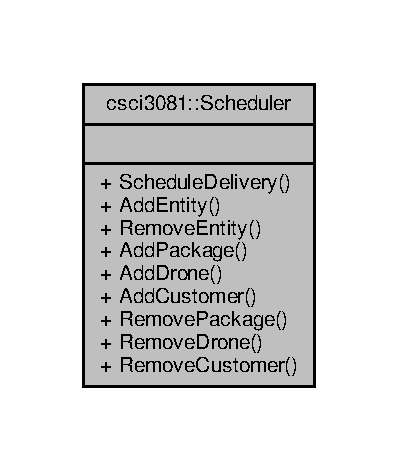
\includegraphics[width=191pt]{classcsci3081_1_1Scheduler__coll__graph}
\end{center}
\end{figure}
\subsection*{Public Member Functions}
\begin{DoxyCompactItemize}
\item 
void \hyperlink{classcsci3081_1_1Scheduler_a06bd24b65f0c52349475eb6ccc661322}{Schedule\+Delivery} (entity\+\_\+project\+::\+Package $\ast$package, entity\+\_\+project\+::\+Customer $\ast$dest, const picojson\+::object \&details)
\begin{DoxyCompactList}\small\item\em Schedules a package delivery to a customer. \end{DoxyCompactList}\item 
\mbox{\Hypertarget{classcsci3081_1_1Scheduler_ab3630723be8af0303181d92079772ef1}\label{classcsci3081_1_1Scheduler_ab3630723be8af0303181d92079772ef1}} 
void \hyperlink{classcsci3081_1_1Scheduler_ab3630723be8af0303181d92079772ef1}{Add\+Entity} (entity\+\_\+project\+::\+Entity $\ast$entity)
\begin{DoxyCompactList}\small\item\em Add an already created entity into the system. \end{DoxyCompactList}\item 
\mbox{\Hypertarget{classcsci3081_1_1Scheduler_a50d8d379859c930d059ef488054b6aac}\label{classcsci3081_1_1Scheduler_a50d8d379859c930d059ef488054b6aac}} 
void \hyperlink{classcsci3081_1_1Scheduler_a50d8d379859c930d059ef488054b6aac}{Remove\+Entity} (entity\+\_\+project\+::\+Entity $\ast$entity)
\begin{DoxyCompactList}\small\item\em Removes an entity from the system. \end{DoxyCompactList}\item 
\mbox{\Hypertarget{classcsci3081_1_1Scheduler_aee6e6c093f5df70acbd8dac37f874876}\label{classcsci3081_1_1Scheduler_aee6e6c093f5df70acbd8dac37f874876}} 
void \hyperlink{classcsci3081_1_1Scheduler_aee6e6c093f5df70acbd8dac37f874876}{Add\+Package} (\hyperlink{classcsci3081_1_1Package}{Package} p)
\begin{DoxyCompactList}\small\item\em Adds a package into the list of Packages. \end{DoxyCompactList}\item 
\mbox{\Hypertarget{classcsci3081_1_1Scheduler_a06957515a2861f5d8213f15466c231a9}\label{classcsci3081_1_1Scheduler_a06957515a2861f5d8213f15466c231a9}} 
void \hyperlink{classcsci3081_1_1Scheduler_a06957515a2861f5d8213f15466c231a9}{Add\+Drone} (\hyperlink{classcsci3081_1_1Drone}{Drone} d)
\begin{DoxyCompactList}\small\item\em Adds a drone into the list of Drones. \end{DoxyCompactList}\item 
\mbox{\Hypertarget{classcsci3081_1_1Scheduler_a6b25bd5bbd478da964960c9175d90032}\label{classcsci3081_1_1Scheduler_a6b25bd5bbd478da964960c9175d90032}} 
void \hyperlink{classcsci3081_1_1Scheduler_a6b25bd5bbd478da964960c9175d90032}{Add\+Customer} (\hyperlink{classcsci3081_1_1Customer}{Customer} c)
\begin{DoxyCompactList}\small\item\em Adds a customer into the list of Customers. \end{DoxyCompactList}\item 
\mbox{\Hypertarget{classcsci3081_1_1Scheduler_a5e1dd1d2bad1d9be7b82a5830efd376f}\label{classcsci3081_1_1Scheduler_a5e1dd1d2bad1d9be7b82a5830efd376f}} 
void \hyperlink{classcsci3081_1_1Scheduler_a5e1dd1d2bad1d9be7b82a5830efd376f}{Remove\+Package} (\hyperlink{classcsci3081_1_1Package}{Package} p)
\begin{DoxyCompactList}\small\item\em Removes a package from the list of Packages. \end{DoxyCompactList}\item 
\mbox{\Hypertarget{classcsci3081_1_1Scheduler_a0b13646a4c8758c4f6baf544a63c79e9}\label{classcsci3081_1_1Scheduler_a0b13646a4c8758c4f6baf544a63c79e9}} 
void \hyperlink{classcsci3081_1_1Scheduler_a0b13646a4c8758c4f6baf544a63c79e9}{Remove\+Drone} (\hyperlink{classcsci3081_1_1Drone}{Drone} d)
\begin{DoxyCompactList}\small\item\em Removes a drone from the list of Drones. \end{DoxyCompactList}\item 
\mbox{\Hypertarget{classcsci3081_1_1Scheduler_ae7d80f81e69926dbc365a8efafe6dc5d}\label{classcsci3081_1_1Scheduler_ae7d80f81e69926dbc365a8efafe6dc5d}} 
void \hyperlink{classcsci3081_1_1Scheduler_ae7d80f81e69926dbc365a8efafe6dc5d}{Remove\+Customer} (\hyperlink{classcsci3081_1_1Customer}{Customer} c)
\begin{DoxyCompactList}\small\item\em Removes a customer from the list of Customers. \end{DoxyCompactList}\end{DoxyCompactItemize}


\subsection{Detailed Description}
A class that stores and handles the entities in the \hyperlink{classcsci3081_1_1DroneSimulation}{Drone\+Simulation} system. 

\subsection{Member Function Documentation}
\mbox{\Hypertarget{classcsci3081_1_1Scheduler_a06bd24b65f0c52349475eb6ccc661322}\label{classcsci3081_1_1Scheduler_a06bd24b65f0c52349475eb6ccc661322}} 
\index{csci3081\+::\+Scheduler@{csci3081\+::\+Scheduler}!Schedule\+Delivery@{Schedule\+Delivery}}
\index{Schedule\+Delivery@{Schedule\+Delivery}!csci3081\+::\+Scheduler@{csci3081\+::\+Scheduler}}
\subsubsection{\texorpdfstring{Schedule\+Delivery()}{ScheduleDelivery()}}
{\footnotesize\ttfamily void csci3081\+::\+Scheduler\+::\+Schedule\+Delivery (\begin{DoxyParamCaption}\item[{entity\+\_\+project\+::\+Package $\ast$}]{package,  }\item[{entity\+\_\+project\+::\+Customer $\ast$}]{dest,  }\item[{const picojson\+::object \&}]{details }\end{DoxyParamCaption})\hspace{0.3cm}{\ttfamily [inline]}}



Schedules a package delivery to a customer. 

Checks each drone in the system and assigns the closest drone to pick up the package and deliver it to the customer. Takes into account the weight of the package and the current capacity of the drones as well, so a drone doesn\textquotesingle{}t get assigned to a package that is too heavy. 

The documentation for this class was generated from the following file\+:\begin{DoxyCompactItemize}
\item 
src/\hyperlink{scheduler_8h}{scheduler.\+h}\end{DoxyCompactItemize}

\chapter{File Documentation}
\hypertarget{customer_8h}{}\section{src/customer.h File Reference}
\label{customer_8h}\index{src/customer.\+h@{src/customer.\+h}}
{\ttfamily \#include $<$string$>$}\newline
{\ttfamily \#include $<$Entity\+Project/\+A\+N\+V\+I\+L/customer.\+h$>$}\newline
Include dependency graph for customer.\+h\+:\nopagebreak
\begin{figure}[H]
\begin{center}
\leavevmode
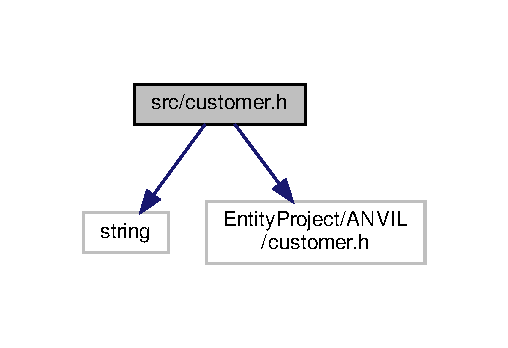
\includegraphics[width=244pt]{customer_8h__incl}
\end{center}
\end{figure}
This graph shows which files directly or indirectly include this file\+:\nopagebreak
\begin{figure}[H]
\begin{center}
\leavevmode
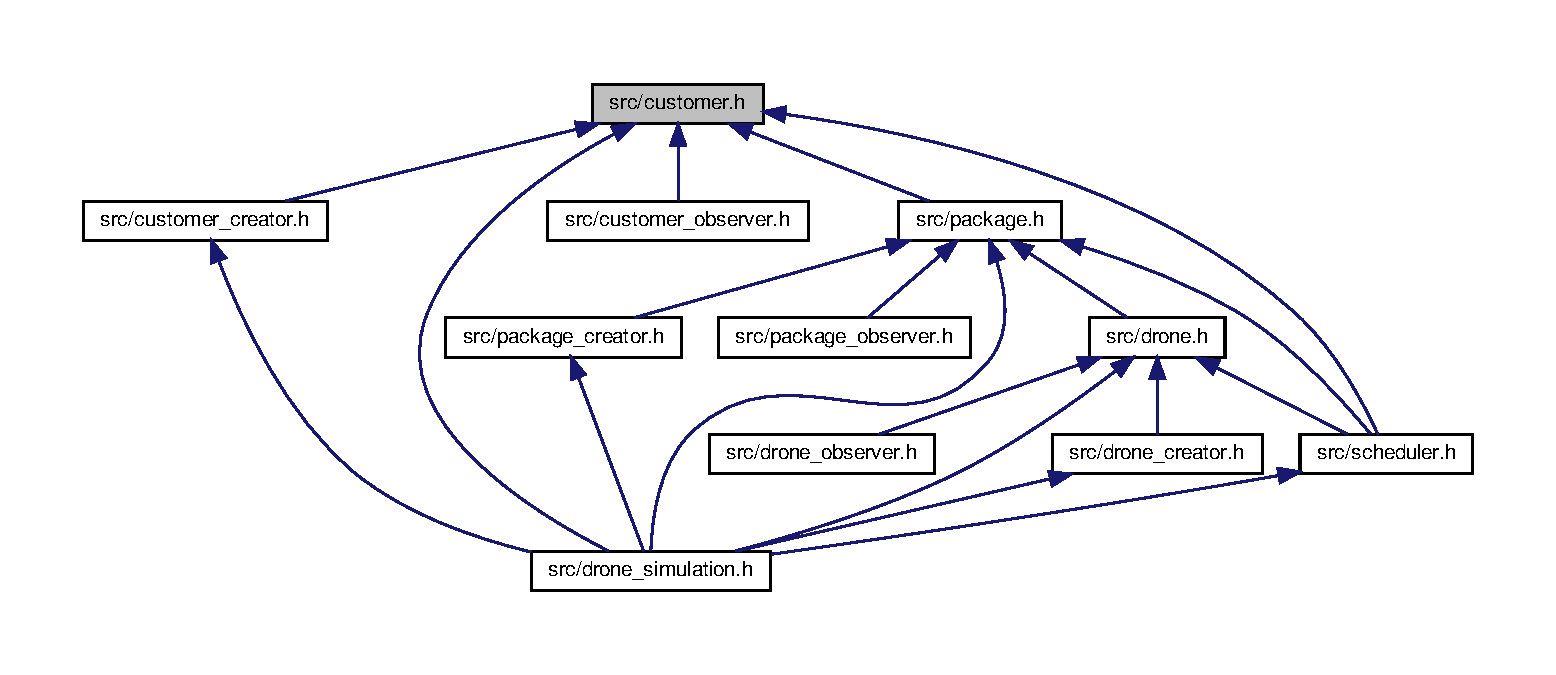
\includegraphics[width=350pt]{customer_8h__dep__incl}
\end{center}
\end{figure}
\subsection*{Classes}
\begin{DoxyCompactItemize}
\item 
class \hyperlink{classcsci3081_1_1Customer}{csci3081\+::\+Customer}
\begin{DoxyCompactList}\small\item\em Stores data about \hyperlink{classcsci3081_1_1Customer}{Customer} entities. \end{DoxyCompactList}\end{DoxyCompactItemize}

\hypertarget{customer__creator_8h}{}\section{src/customer\+\_\+creator.h File Reference}
\label{customer__creator_8h}\index{src/customer\+\_\+creator.\+h@{src/customer\+\_\+creator.\+h}}
{\ttfamily \#include $<$project/src/customer.\+h$>$}\newline
{\ttfamily \#include $<$project/src/entity\+\_\+creator.\+h$>$}\newline
Include dependency graph for customer\+\_\+creator.\+h\+:\nopagebreak
\begin{figure}[H]
\begin{center}
\leavevmode
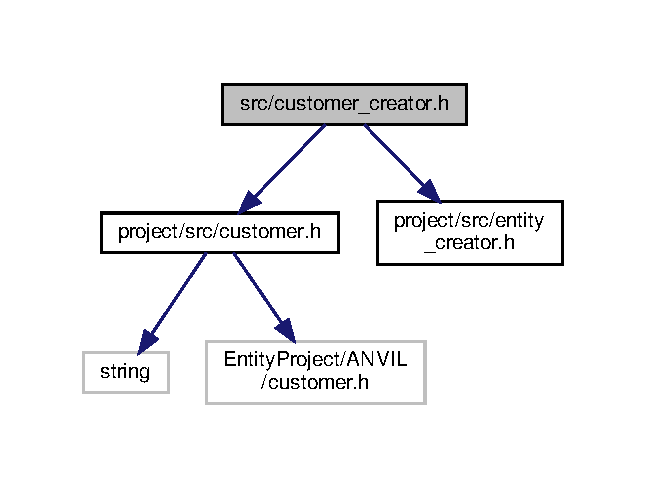
\includegraphics[width=310pt]{customer__creator_8h__incl}
\end{center}
\end{figure}
This graph shows which files directly or indirectly include this file\+:\nopagebreak
\begin{figure}[H]
\begin{center}
\leavevmode
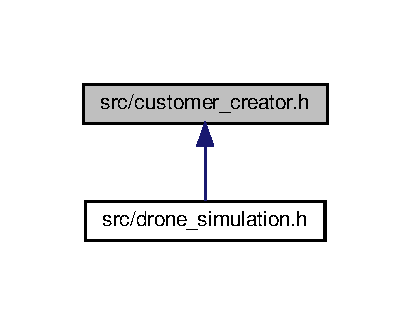
\includegraphics[width=197pt]{customer__creator_8h__dep__incl}
\end{center}
\end{figure}
\subsection*{Classes}
\begin{DoxyCompactItemize}
\item 
class \hyperlink{classcsci3081_1_1CustomerCreator}{csci3081\+::\+Customer\+Creator}
\begin{DoxyCompactList}\small\item\em A class that creates a \hyperlink{classcsci3081_1_1Customer}{Customer} object. \end{DoxyCompactList}\end{DoxyCompactItemize}

\hypertarget{customer__observer_8h}{}\section{src/customer\+\_\+observer.h File Reference}
\label{customer__observer_8h}\index{src/customer\+\_\+observer.\+h@{src/customer\+\_\+observer.\+h}}
{\ttfamily \#include $<$project/src/entity\+\_\+observer.\+h$>$}\newline
{\ttfamily \#include $<$project/src/customer.\+h$>$}\newline
{\ttfamily \#include $<$vector$>$}\newline
{\ttfamily \#include $<$string$>$}\newline
Include dependency graph for customer\+\_\+observer.\+h\+:\nopagebreak
\begin{figure}[H]
\begin{center}
\leavevmode
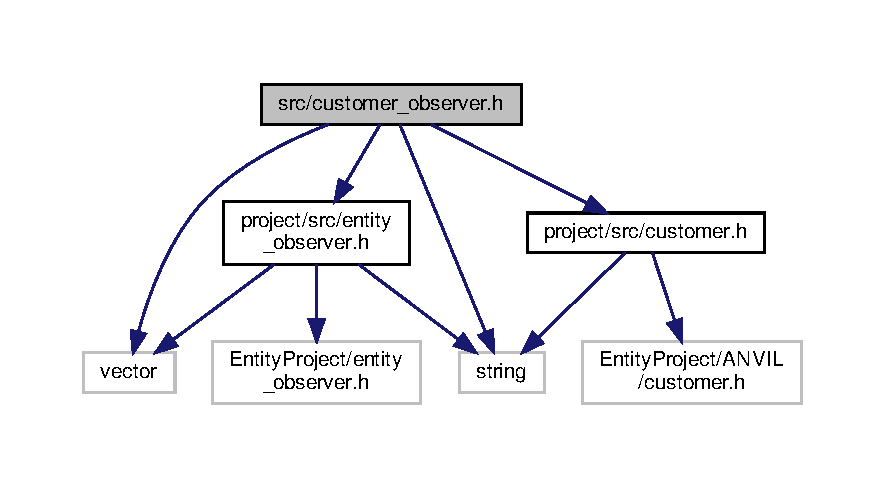
\includegraphics[width=350pt]{customer__observer_8h__incl}
\end{center}
\end{figure}
\subsection*{Classes}
\begin{DoxyCompactItemize}
\item 
class \hyperlink{classcsci3081_1_1CustomerObserver}{csci3081\+::\+Customer\+Observer}
\begin{DoxyCompactList}\small\item\em implements \hyperlink{classcsci3081_1_1Customer}{Customer} observer \end{DoxyCompactList}\end{DoxyCompactItemize}

\hypertarget{drone_8h}{}\section{src/drone.h File Reference}
\label{drone_8h}\index{src/drone.\+h@{src/drone.\+h}}
{\ttfamily \#include $<$stdlib.\+h$>$}\newline
{\ttfamily \#include $<$time.\+h$>$}\newline
{\ttfamily \#include $<$string$>$}\newline
{\ttfamily \#include $<$vector$>$}\newline
{\ttfamily \#include $<$Entity\+Project/\+A\+N\+V\+I\+L/drone.\+h$>$}\newline
{\ttfamily \#include $<$project/src/package.\+h$>$}\newline
Include dependency graph for drone.\+h\+:\nopagebreak
\begin{figure}[H]
\begin{center}
\leavevmode
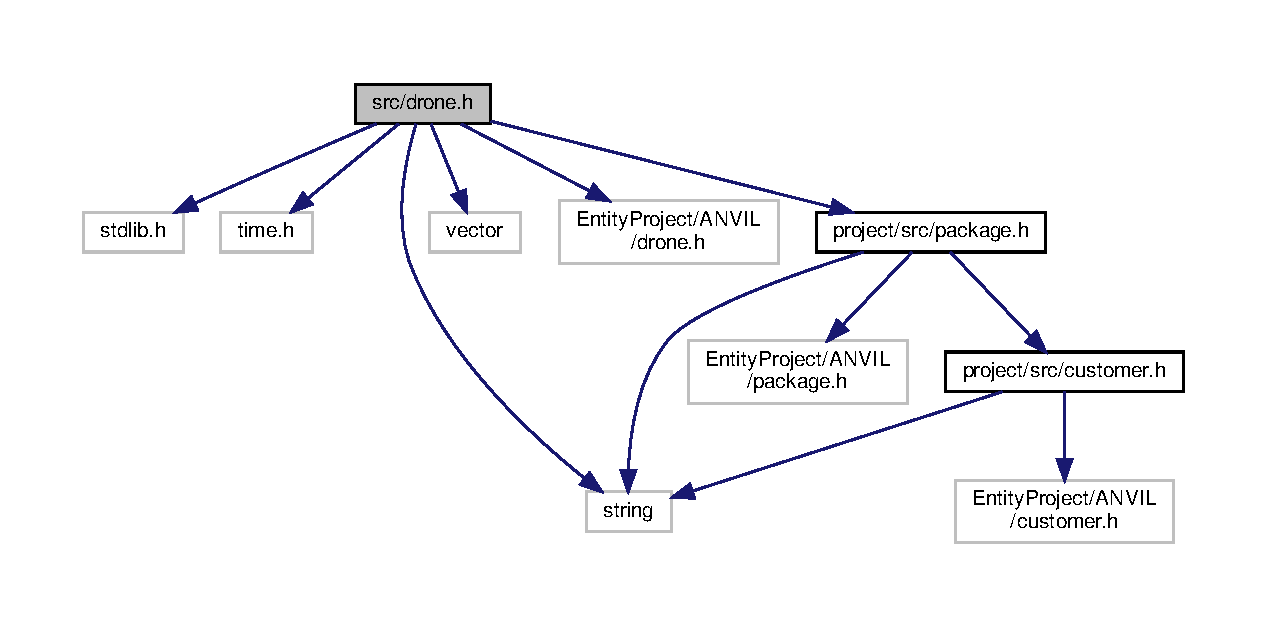
\includegraphics[width=350pt]{drone_8h__incl}
\end{center}
\end{figure}
This graph shows which files directly or indirectly include this file\+:\nopagebreak
\begin{figure}[H]
\begin{center}
\leavevmode
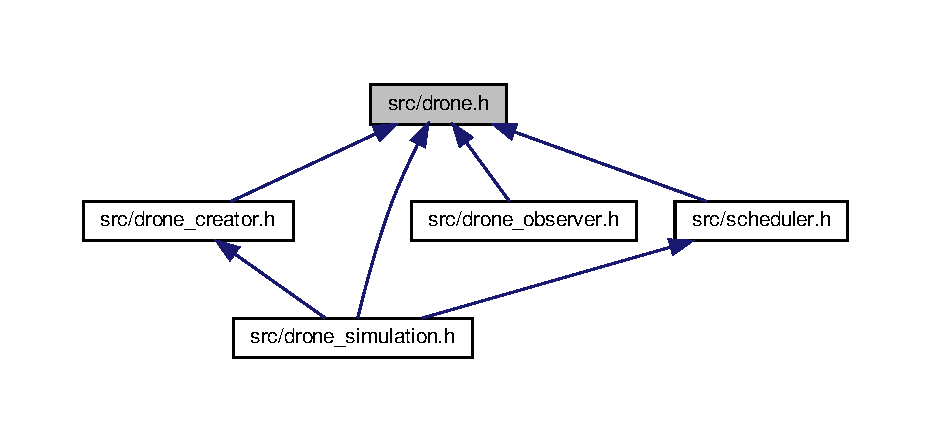
\includegraphics[width=350pt]{drone_8h__dep__incl}
\end{center}
\end{figure}
\subsection*{Classes}
\begin{DoxyCompactItemize}
\item 
class \hyperlink{classcsci3081_1_1Drone}{csci3081\+::\+Drone}
\begin{DoxyCompactList}\small\item\em Stores data about \hyperlink{classcsci3081_1_1Drone}{Drone} entities. \end{DoxyCompactList}\end{DoxyCompactItemize}

\hypertarget{drone__creator_8h}{}\section{src/drone\+\_\+creator.h File Reference}
\label{drone__creator_8h}\index{src/drone\+\_\+creator.\+h@{src/drone\+\_\+creator.\+h}}
{\ttfamily \#include $<$project/src/drone.\+h$>$}\newline
{\ttfamily \#include $<$project/src/entity\+\_\+creator.\+h$>$}\newline
Include dependency graph for drone\+\_\+creator.\+h\+:\nopagebreak
\begin{figure}[H]
\begin{center}
\leavevmode
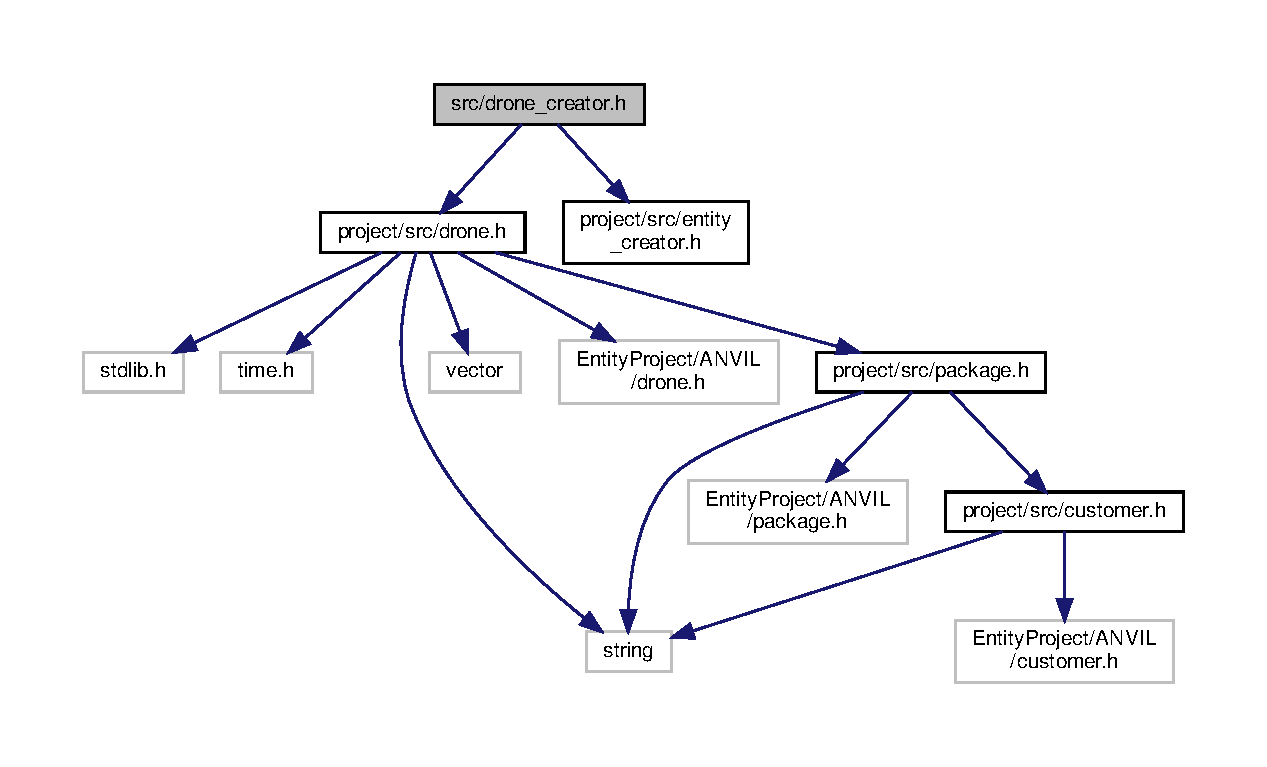
\includegraphics[width=350pt]{drone__creator_8h__incl}
\end{center}
\end{figure}
This graph shows which files directly or indirectly include this file\+:\nopagebreak
\begin{figure}[H]
\begin{center}
\leavevmode
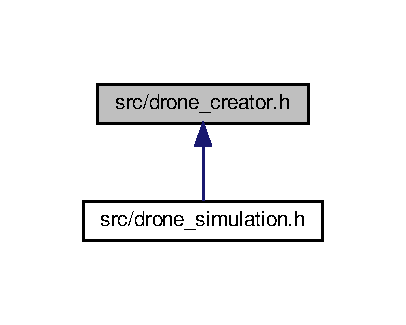
\includegraphics[width=195pt]{drone__creator_8h__dep__incl}
\end{center}
\end{figure}
\subsection*{Classes}
\begin{DoxyCompactItemize}
\item 
class \hyperlink{classcsci3081_1_1DroneCreator}{csci3081\+::\+Drone\+Creator}
\begin{DoxyCompactList}\small\item\em A class that creates a \hyperlink{classcsci3081_1_1Drone}{Drone} object. \end{DoxyCompactList}\end{DoxyCompactItemize}

\hypertarget{drone__observer_8h}{}\section{src/drone\+\_\+observer.h File Reference}
\label{drone__observer_8h}\index{src/drone\+\_\+observer.\+h@{src/drone\+\_\+observer.\+h}}
{\ttfamily \#include $<$project/src/entity\+\_\+observer.\+h$>$}\newline
{\ttfamily \#include $<$project/src/drone.\+h$>$}\newline
{\ttfamily \#include $<$vector$>$}\newline
{\ttfamily \#include $<$string$>$}\newline
Include dependency graph for drone\+\_\+observer.\+h\+:\nopagebreak
\begin{figure}[H]
\begin{center}
\leavevmode
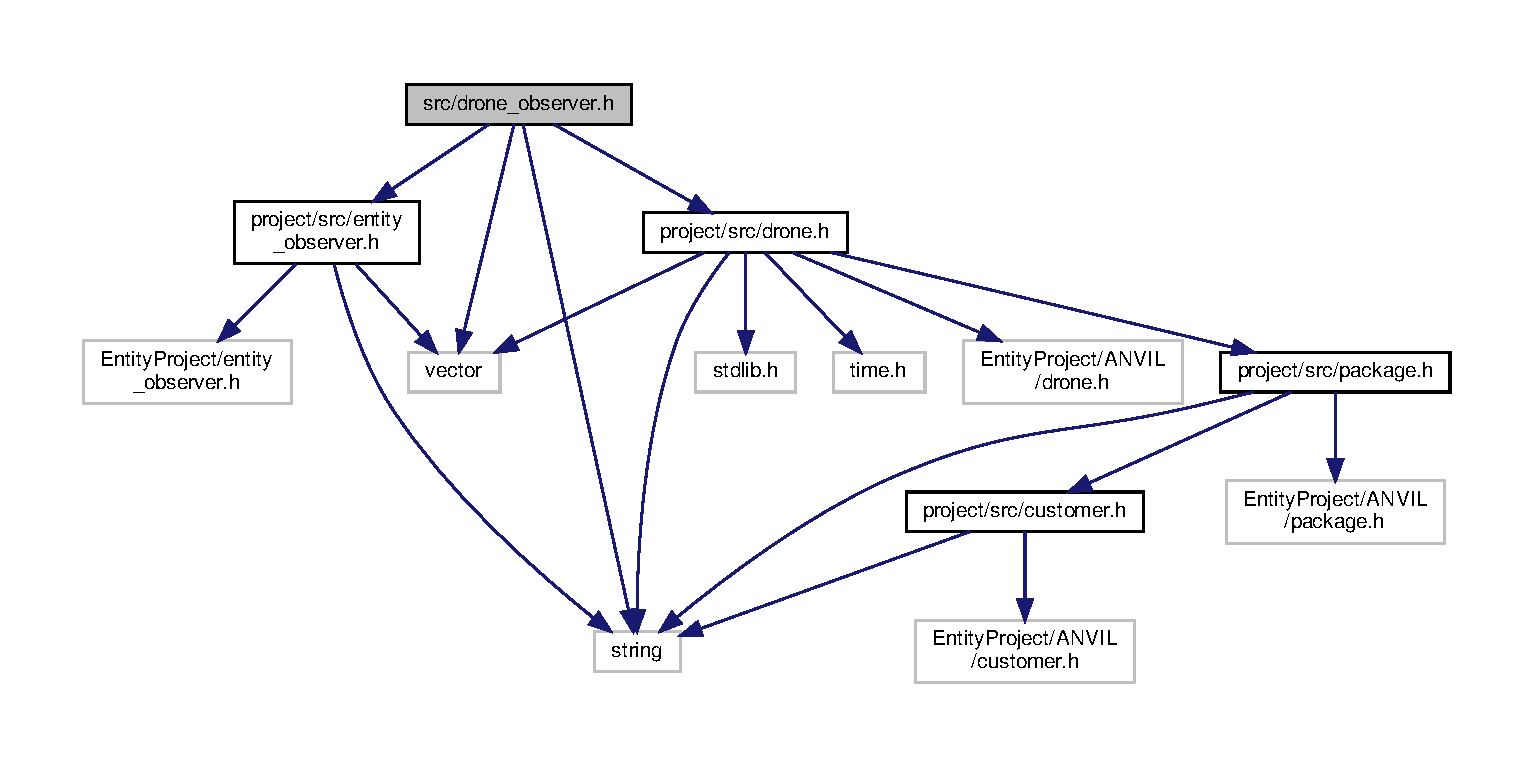
\includegraphics[width=350pt]{drone__observer_8h__incl}
\end{center}
\end{figure}
\subsection*{Classes}
\begin{DoxyCompactItemize}
\item 
class \hyperlink{classcsci3081_1_1DroneObserver}{csci3081\+::\+Drone\+Observer}
\begin{DoxyCompactList}\small\item\em implements \hyperlink{classcsci3081_1_1Drone}{Drone} observer \end{DoxyCompactList}\end{DoxyCompactItemize}

\hypertarget{drone__simulation_8h}{}\section{src/drone\+\_\+simulation.h File Reference}
\label{drone__simulation_8h}\index{src/drone\+\_\+simulation.\+h@{src/drone\+\_\+simulation.\+h}}
{\ttfamily \#include $<$Entity\+Project/\+A\+N\+V\+I\+L/drone\+\_\+delivery\+\_\+system.\+h$>$}\newline
{\ttfamily \#include $<$Entity\+Project/../picojson.\+h$>$}\newline
{\ttfamily \#include $<$project/src/drone.\+h$>$}\newline
{\ttfamily \#include $<$project/src/customer.\+h$>$}\newline
{\ttfamily \#include $<$project/src/package.\+h$>$}\newline
{\ttfamily \#include $<$project/src/scheduler.\+h$>$}\newline
{\ttfamily \#include $<$project/src/customer\+\_\+creator.\+h$>$}\newline
{\ttfamily \#include $<$project/src/drone\+\_\+creator.\+h$>$}\newline
{\ttfamily \#include $<$project/src/package\+\_\+creator.\+h$>$}\newline
{\ttfamily \#include $<$vector$>$}\newline
{\ttfamily \#include $<$string$>$}\newline
Include dependency graph for drone\+\_\+simulation.\+h\+:\nopagebreak
\begin{figure}[H]
\begin{center}
\leavevmode
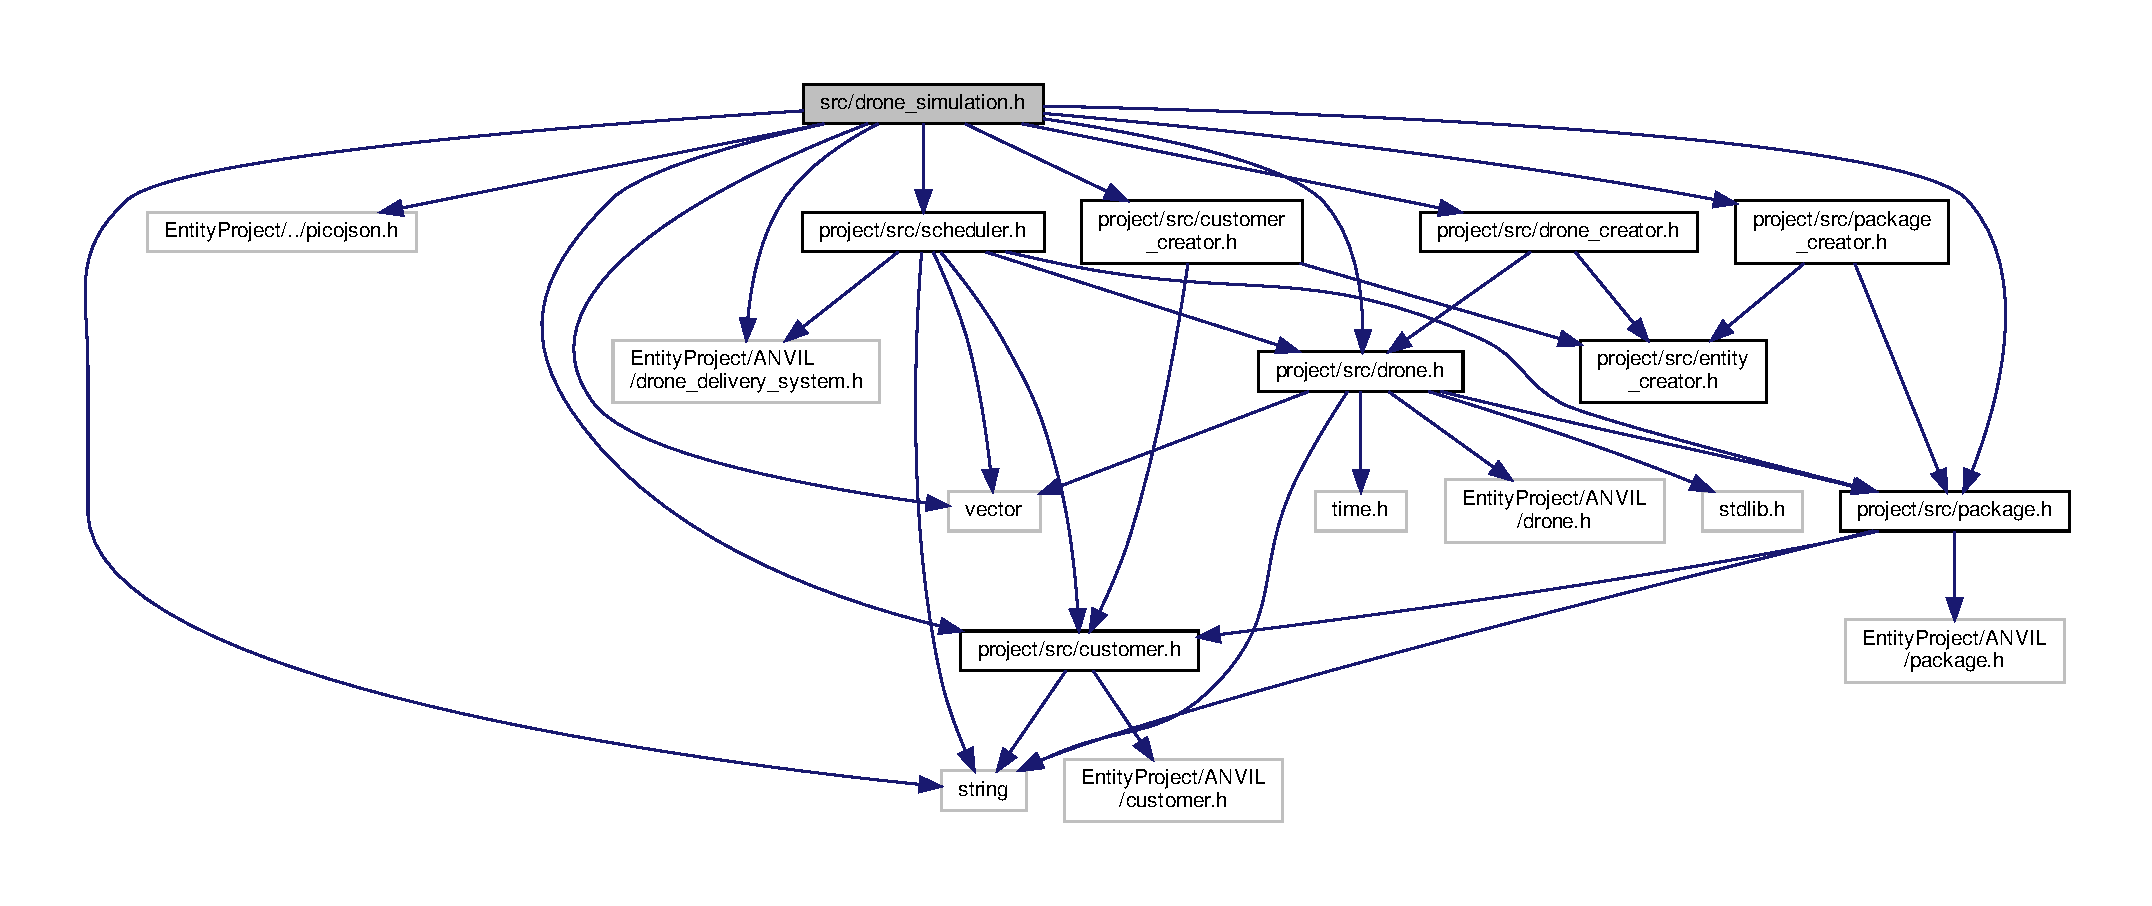
\includegraphics[width=350pt]{drone__simulation_8h__incl}
\end{center}
\end{figure}
\subsection*{Classes}
\begin{DoxyCompactItemize}
\item 
class \hyperlink{classcsci3081_1_1DroneSimulation}{csci3081\+::\+Drone\+Simulation}
\begin{DoxyCompactList}\small\item\em A facade class that implements the \hyperlink{classcsci3081_1_1Drone}{Drone} Delivery System. \end{DoxyCompactList}\end{DoxyCompactItemize}

\hypertarget{entity__creator_8h}{}\section{src/entity\+\_\+creator.h File Reference}
\label{entity__creator_8h}\index{src/entity\+\_\+creator.\+h@{src/entity\+\_\+creator.\+h}}
This graph shows which files directly or indirectly include this file\+:\nopagebreak
\begin{figure}[H]
\begin{center}
\leavevmode
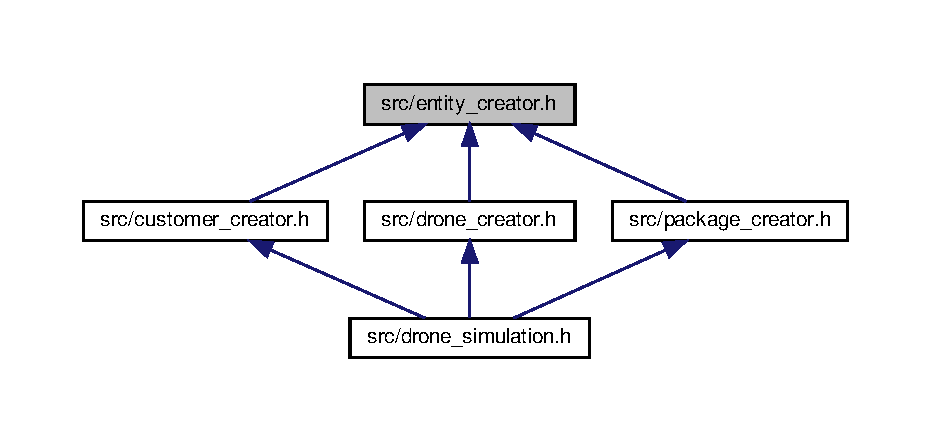
\includegraphics[width=350pt]{entity__creator_8h__dep__incl}
\end{center}
\end{figure}
\subsection*{Classes}
\begin{DoxyCompactItemize}
\item 
class \hyperlink{classcsci3081_1_1EntityCreator}{csci3081\+::\+Entity\+Creator}
\begin{DoxyCompactList}\small\item\em An abstract class that creates entities. \end{DoxyCompactList}\end{DoxyCompactItemize}

\hypertarget{entity__observer_8h}{}\section{src/entity\+\_\+observer.h File Reference}
\label{entity__observer_8h}\index{src/entity\+\_\+observer.\+h@{src/entity\+\_\+observer.\+h}}
{\ttfamily \#include $<$Entity\+Project/entity\+\_\+observer.\+h$>$}\newline
{\ttfamily \#include $<$vector$>$}\newline
{\ttfamily \#include $<$string$>$}\newline
Include dependency graph for entity\+\_\+observer.\+h\+:\nopagebreak
\begin{figure}[H]
\begin{center}
\leavevmode
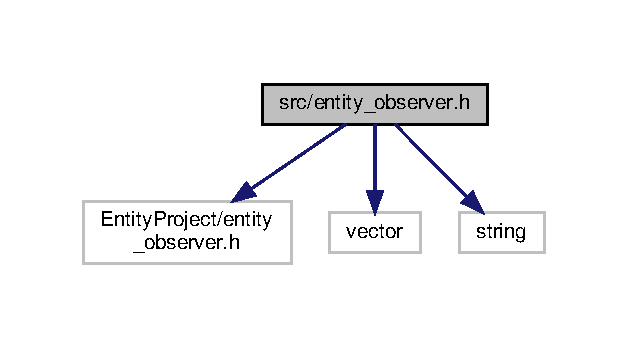
\includegraphics[width=302pt]{entity__observer_8h__incl}
\end{center}
\end{figure}
This graph shows which files directly or indirectly include this file\+:\nopagebreak
\begin{figure}[H]
\begin{center}
\leavevmode
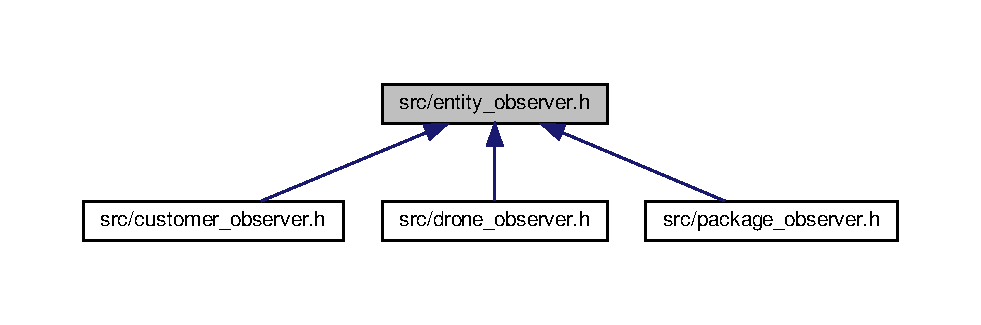
\includegraphics[width=350pt]{entity__observer_8h__dep__incl}
\end{center}
\end{figure}
\subsection*{Classes}
\begin{DoxyCompactItemize}
\item 
class \hyperlink{classcsci3081_1_1EntityObserver}{csci3081\+::\+Entity\+Observer}
\begin{DoxyCompactList}\small\item\em An abstract class from which specialized entity observers inherit from. \end{DoxyCompactList}\end{DoxyCompactItemize}

\hypertarget{package__creator_8h}{}\section{src/package\+\_\+creator.h File Reference}
\label{package__creator_8h}\index{src/package\+\_\+creator.\+h@{src/package\+\_\+creator.\+h}}
{\ttfamily \#include $<$project/src/package.\+h$>$}\newline
{\ttfamily \#include $<$project/src/entity\+\_\+creator.\+h$>$}\newline
Include dependency graph for package\+\_\+creator.\+h\+:\nopagebreak
\begin{figure}[H]
\begin{center}
\leavevmode
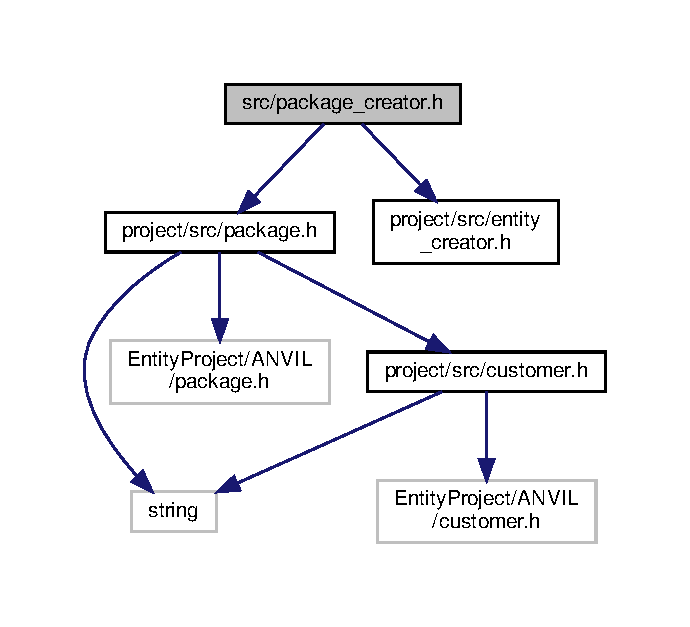
\includegraphics[width=331pt]{package__creator_8h__incl}
\end{center}
\end{figure}
This graph shows which files directly or indirectly include this file\+:\nopagebreak
\begin{figure}[H]
\begin{center}
\leavevmode
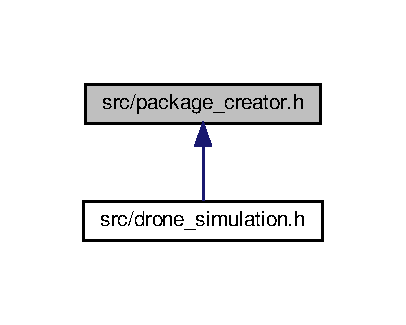
\includegraphics[width=195pt]{package__creator_8h__dep__incl}
\end{center}
\end{figure}
\subsection*{Classes}
\begin{DoxyCompactItemize}
\item 
class \hyperlink{classcsci3081_1_1PackageCreator}{csci3081\+::\+Package\+Creator}
\begin{DoxyCompactList}\small\item\em A class that creates a \hyperlink{classcsci3081_1_1Package}{Package} object. \end{DoxyCompactList}\end{DoxyCompactItemize}

\hypertarget{package__observer_8h}{}\section{src/package\+\_\+observer.h File Reference}
\label{package__observer_8h}\index{src/package\+\_\+observer.\+h@{src/package\+\_\+observer.\+h}}
{\ttfamily \#include $<$project/src/entity\+\_\+observer.\+h$>$}\newline
{\ttfamily \#include $<$project/src/package.\+h$>$}\newline
{\ttfamily \#include $<$vector$>$}\newline
{\ttfamily \#include $<$string$>$}\newline
Include dependency graph for package\+\_\+observer.\+h\+:\nopagebreak
\begin{figure}[H]
\begin{center}
\leavevmode
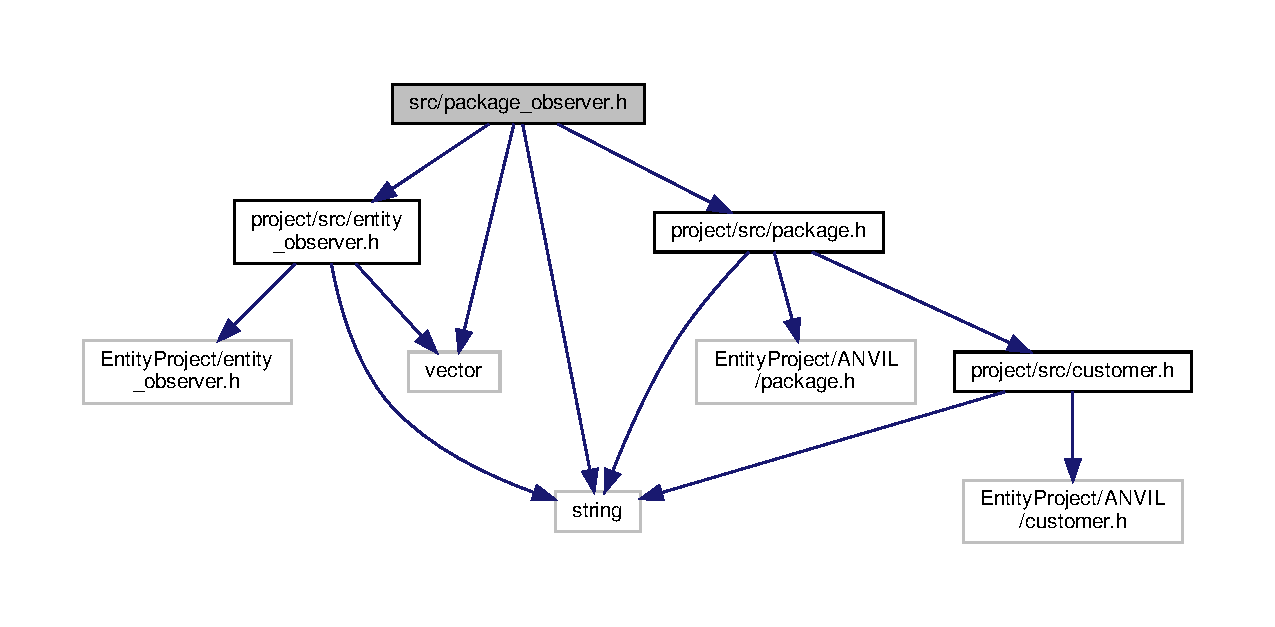
\includegraphics[width=350pt]{package__observer_8h__incl}
\end{center}
\end{figure}
\subsection*{Classes}
\begin{DoxyCompactItemize}
\item 
class \hyperlink{classcsci3081_1_1PackageObserver}{csci3081\+::\+Package\+Observer}
\begin{DoxyCompactList}\small\item\em implements \hyperlink{classcsci3081_1_1Package}{Package} observer \end{DoxyCompactList}\end{DoxyCompactItemize}

\hypertarget{scheduler_8h}{}\section{src/scheduler.h File Reference}
\label{scheduler_8h}\index{src/scheduler.\+h@{src/scheduler.\+h}}
{\ttfamily \#include $<$Entity\+Project/\+A\+N\+V\+I\+L/drone\+\_\+delivery\+\_\+system.\+h$>$}\newline
{\ttfamily \#include $<$project/src/drone.\+h$>$}\newline
{\ttfamily \#include $<$project/src/customer.\+h$>$}\newline
{\ttfamily \#include $<$project/src/package.\+h$>$}\newline
{\ttfamily \#include $<$vector$>$}\newline
{\ttfamily \#include $<$string$>$}\newline
Include dependency graph for scheduler.\+h\+:\nopagebreak
\begin{figure}[H]
\begin{center}
\leavevmode
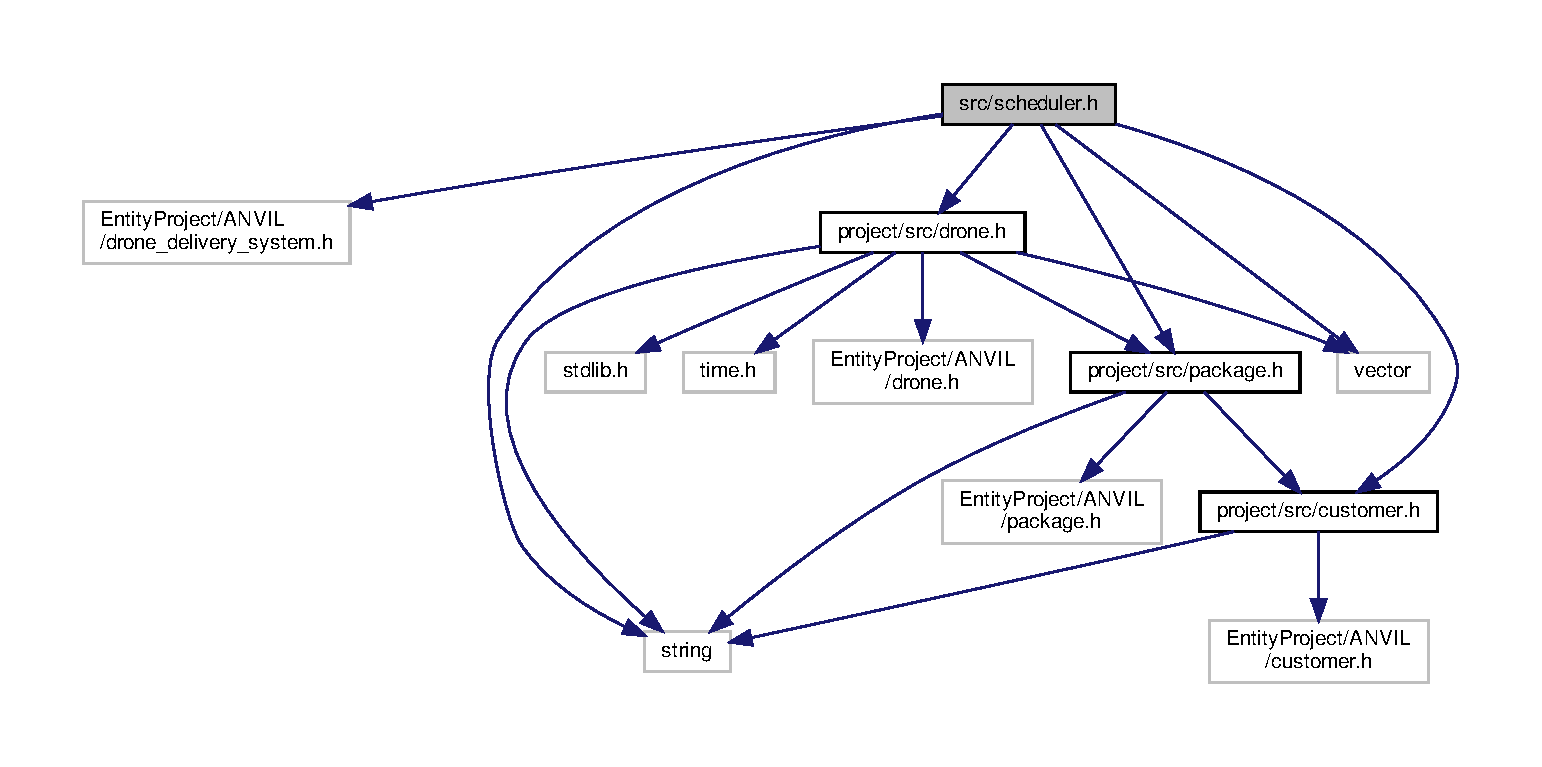
\includegraphics[width=350pt]{scheduler_8h__incl}
\end{center}
\end{figure}
This graph shows which files directly or indirectly include this file\+:\nopagebreak
\begin{figure}[H]
\begin{center}
\leavevmode
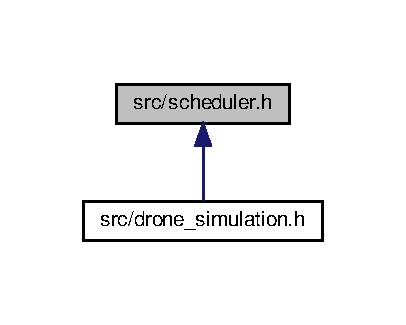
\includegraphics[width=195pt]{scheduler_8h__dep__incl}
\end{center}
\end{figure}
\subsection*{Classes}
\begin{DoxyCompactItemize}
\item 
class \hyperlink{classcsci3081_1_1Scheduler}{csci3081\+::\+Scheduler}
\begin{DoxyCompactList}\small\item\em A class that stores and handles the entities in the \hyperlink{classcsci3081_1_1DroneSimulation}{Drone\+Simulation} system. \end{DoxyCompactList}\end{DoxyCompactItemize}

%--- End generated contents ---

% Index
\backmatter
\newpage
\phantomsection
\clearemptydoublepage
\addcontentsline{toc}{chapter}{Index}
\printindex

\end{document}
